\documentclass[12pt,oneside]{book}
\usepackage{graphicx}
\usepackage{subcaption}
\usepackage{color}
\usepackage{amscd,amsfonts,amssymb,amsmath,amsthm}
\usepackage[utf8]{inputenc}
\usepackage[T1]{fontenc}
\usepackage[english]{babel}
\usepackage[all]{xy}
\usepackage{enumerate}
\usepackage[a4paper]{geometry}
\usepackage{fancyhdr}
\usepackage{tabularx}
\usepackage{makeidx}
\usepackage[backend=biber,style=numeric,sorting=nyt]{biblatex}
\usepackage{hyperref}
\usepackage{xcolor}

\definecolor{navyblue}{rgb}{0.0, 0.0, 0.5}

\addbibresource{referencias.bib}

\geometry{textwidth=150mm,textheight=247mm,top=30mm,bottom=30mm,left=30mm,right=30mm,headsep=10mm,
footskip=10mm}


\pagestyle{fancy}
\fancyhead[LO]{\rightmark}
\fancyhead[RO]{\thepage}
\fancyfoot[C]{\empty}

\makeindex

\newtheorem{defi}   {Definition}[chapter]
\newtheorem{teo}    {Theorem}[chapter]
\newtheorem{ex}     {Example}[chapter]
\newtheorem{prop}   {Proposition}[chapter]
\newtheorem{lem}    {Lemma}[chapter]
\newtheorem{cor}    {Corollary}[chapter]
\newtheorem{obs}    {Observation}[chapter]
\newtheorem{conj}	{Conjecture}

\newcommand{\ds}{\displaystyle}
\newcommand{\R}{\mathbb{R}}
\newcommand{\RP}{\mathbb{R}P}
\newcommand{\Z}{\mathbb{Z}}
\newcommand{\F}{\mathbb{F}}
\newcommand{\ccup}{\smile}
\newcommand{\ccap}{\frown}
\newcommand{\tensor}{\otimes}
\newcommand{\wt}{\widetilde}





\begin{document}





    \fontfamily{ptm}\selectfont

    \begin{titlepage}
        \begin{center}
            \textbf{FEDERAL UNIVERSITY OF SÃO CARLOS}
        \end{center}

        \vspace{-0.8cm}

        \begin{center}  
            \fontsize{10}{12}\selectfont CENTER OF EXACT SCIENCES AND TECHNOLOGY
        \end{center}

        \vspace{-0.8cm}

        \begin{center}
            \fontsize{10}{12}\selectfont GRADUATE PROGRAM IN MATHEMATICS
        \end{center}

        \vspace{3cm}

        \begin{center}
            \small{Alex Melges Barbosa}
        \end{center}

        \vspace{3cm}

        \begin{center}
            \Large{\textbf{Characteristic Classes of \\ Topological and Generalized Manifolds}}
        \end{center}

        \vspace{10cm}

        \begin{center}
            São Carlos - SP/Brazil
        \end{center}

        \vspace{-0.8cm}

        \begin{center}
            2022
        \end{center}
    \end{titlepage}



    \newpage
    \thispagestyle{empty}

    \begin{center}
        \small{Alex Melges Barbosa}

        \scriptsize{\href{mailto:exemplo@dominio.com}{\textcolor{navyblue}{melges.ab@gmail.com}}}

        \scriptsize{\href{https://www.linkedin.com/in/alexmelgesbarbosa/}{ \textcolor{navyblue}{LinkedIn profile}}}

        \scriptsize{\href{https://github.com/alex-melges}{\textcolor{navyblue}{GitHub profile}}}
    \end{center}

    \vspace{3cm}

    \begin{center}
        \Large{\textbf{Characteristic Classes of \\ Topological and Generalized Manifolds}}
    \end{center}

    \vspace{2cm}

    \begin{flushright}
        \begin{minipage}{0.55\textwidth}
            Thesis submitted to the Graduate Program in Mathematics at the Federal University of 
            São Carlos as part of the requirements for the degree of PhD in Mathematics \\[0.5cm] 
            Advisor: Prof. Dr. Edivaldo Lopes dos Santos

            \hspace{1.7cm}\scriptsize{\href{mailto:exemplo@dominio.com}{\textcolor{navyblue}{edivaldo@ufscar.br}}}
        \end{minipage}
    \end{flushright}

    \vfill

    \begin{center}
        São Carlos - SP/Brazil
    \end{center}

    \vspace{-0.8cm}

    \begin{center}
        03/24/2022
    \end{center}



    \newpage
    \thispagestyle{empty}

    \vspace{\fill}

    \begin{flushright}
        \begin{minipage}{5cm}
            \begin{flushright}
                \vspace{22cm}\textit{To my parents \\ Antonio Carlos and Edith \\ and my siblings \\ 
                Carol and André.}
            \end{flushright}
        \end{minipage}
    \end{flushright}



    \newpage
    \chapter*{Acknowledgements}
    \thispagestyle{empty}
    \

    First of all, I would like to thank God for the opportunities and doors that have opened throughout 
    my 11-year academic journey, spanning my undergraduate, master’s, and doctoral degrees. There have 
    been many moments—both good and challenging—that have shaped me into the person and professional I 
    am today.

    I would also like to express my gratitude to my parents, Antonio Carlos and Edith, and my siblings, 
    Carol and André, who have been my unwavering support every day.

    A special thanks goes to two individuals who have been my mentors throughout this process: Edivaldo 
    and João Peres. They have not only helped shape me into the mathematician I am today but, more 
    importantly, have played a key role in shaping the person I’ve become. Thank you both very much.

    Last but not least, I want to thank my friends, who have been like a second family to me during this 
    long journey. There’s no need for me to mention them by name, as only those who have lifted me up 
    during my stumbles and celebrated my successes with me truly understand the depth of my gratitude 
    and affection for them.

    This work was supported financially by CAPES.



    \vspace{2cm}

    \begin{center}
        \begin{minipage}{10cm}
            \textit{In memory of my father, Antonio Carlos Barbosa. Unfortunately, you couldn't be 
            physically present on the day of my defense, but you certainly were and will always be 
            present in the hearts of our entire family. Thank you for everything!}
        \end{minipage}
    \end{center}



    \newpage
    \thispagestyle{empty}

    \begin{flushright}
        \begin{minipage}{7cm}
            \begin{flushright}
                \vspace{22cm}\textit{Either you have a strategy, or you're part of someone else's 
                strategy.}

                \vspace{0.2cm} Alvin Toffler
            \end{flushright}
        \end{minipage}
    \end{flushright}



    \chapter*{Abstract}
    \thispagestyle{empty}

    In this work, we will first present generalized bundles, a concept developed by Fadell with the aim 
    of generalizing vector bundles, Stiefel-Whitney classes, and Wu's formula from the context of smooth 
    manifolds to topological manifolds. After that, we will use generalized bundles to obtain original 
    results concerning the Thom, Stiefel-Whitney, Wu, and Euler classes of topological manifolds, as 
    well as to provide a second proof of Wu's formula for topological manifolds and to establish the 
    topological version of the Poincaré-Hopf Theorem. Finally, we will use Poincaré and 
    Poincaré-Lefschetz dualities to construct the Stiefel-Whitney classes of generalized manifolds in a 
    broader manner, aiming to present, for the first time in the literature, a proof of Wu's formula 
    for such manifolds.

    \

    \noindent Keywords: characteristic classes, generalized bundles, topological manifolds, generalized 
    manifolds, Wu's formula.



    \tableofcontents
    \thispagestyle{empty}

    \listoffigures
    \thispagestyle{empty}



    \chapter*{List of Notations}
    \thispagestyle{empty}

    \begin{enumerate}
        \item Saying that $f:X\to Y$ is a map means the same as saying that $f$ is a continuous function 
        between topological spaces.
        \item $f:X \rightleftarrows Y:g$ denotes two maps when $f:X\to Y$ and $g:Y\to X$, not necessarily 
        inverses of each other. 
        \item $1:X\to X$ denotes the identity map on $X$.
        \item $f^{-1}$ denotes the preimage of a map $f$, as well as its inverse mapping (when it exists).
        \item If $f:X\to Y$ is a map, then $f(\_)$ denotes $f(x)$ for every $x\in X$.
        \item If $H:X\times Y\to Z$ is a map defined on a Cartesian product, then $H(\_,y)$ denotes 
        $H(x,y)$ for every $x\in X$. The same holds for $H(x,\_)$.
        \item $p_{i}:X_{1}\times \cdots\times X_{n}\to X_{i}$ denotes the projection on the $i$-th factor.
        \item $d:X\to X\times X$ denotes the diagonal map\index{diagonal!map} given by $d(x)=(x,x)$.
        \item Saying that $U\subset X$ is an open neighborhood of some subset $A\subset X$ means the 
        same as saying that $U$ is an open subspace of $X$ that contains $A$.
        \item Saying that $\mathcal{U}$ is an open cover of a topological space $B$ means the same as 
        saying that $\mathcal{U}=\{ U\subset B \}$, such that $U\subset B$ is an open subspace of $B$ 
        for every $U\in\mathcal{U}$ and $\ds\bigcup_{U\in\mathcal{U}}U=B$.  
        \item $X \approx Y$ denotes when two topological spaces are homeomorphic.
        \item $f \sim g$ denotes when two maps are homotopic.
        \item $X\sim Y$ denotes when two topological spaces have the same type of homotopy.
        \item $G_{1}\cong G_{2}$ denotes when two algebraic objects are, appropriately, isomorphic.
        \item $\mathbb{S}^{n-1}=\{ x\in\R^{n} \ : \ \| x \|=1 \}$.
        \item $D^{n}=\{ x\in\R^{n} \ : \ \| x \|\leq1 \}$.
        \item $B^{n}=\{ x\in\R^{n} \ : \ \| x \|<1 \}$.
        \item $I=[0,1]\subset \R$.
        \item $X^{I}$ denotes the topological space of paths in $X$.
        \item $\Omega(X,x_{0})=\{ \omega\in X^{I} \ : \ \omega(0)=\omega(1)=x_{0} \}$.
        \item $H_{k}(X,A;R)$ and $H^{k}(X,A;R)$ denote the $k$-th $R$-modules of singular homology and 
        cohomology, respectively, of the pair $(X,A)$ with coefficients in a commutative ring $R$ with 
        unity.
        \item $H_{k}^{c}(X,A;R)$ and $H^{k}_{c}(X,A;R)$ denote, respectively, the $k$-th $R$-modules of 
        singular homology and cohomology with compact support.
        \item $\wt{H}_{k}(X,A;R)$ and $\wt{H}^{k}(X,A;R)$ denote, respectively, the $k$-th $R$-modules of 
        reduced singular homology and cohomology.
        \item $\check{H}^{k}(X,A;R)$ denotes the $k$-th $R$-module of Čech cohomology.
        \item $H^{k}(X,A;R)=(x)$ denotes that the $k$-th $R$-module of cohomology of the pair $(X,A)$ is 
        generated by the element $x\in H^{k}(X,A;R)$. The same applies for homology modules.
        \item If $x\in H^{k}(X,A;R)$, then we denote $|x|=k$. The same applies for homology modules.
        \item $<,>:H^{k}(X,A;R)\tensor H_{k}(X,A;R)\to R$ denotes the Kronecker product, which maps 
        $\varphi\tensor\sigma\mapsto <\varphi,\sigma>$.
        \item $\ccap:H_{k}(X,A\cup B;R)\tensor H^{l}(X,A;R)\to H_{k-l}(X,B;R)$ denotes the cap product, 
        which maps $\sigma\tensor\varphi\mapsto\sigma\ccap\varphi$.
        \item $\ccup:H^{k}(X,A;R)\tensor H^{l}(X,B;R)\to H^{k+l}(X,A\cup B;R)$ denotes the cup product, 
        which maps $\varphi\tensor\psi\mapsto\varphi\ccup\psi$.
        \item $\times:H^{k}(X,A;R)\tensor H^{l}(Y,B;R)\to H^{k+l}(X\times Y,(X\times B)\cup(A\times Y);R)$ 
        denotes the cross product, which maps $\varphi\tensor\psi\mapsto\varphi\times\psi$.
        \thispagestyle{empty}
    \end{enumerate}



    \chapter{Introduction}
    \thispagestyle{empty}

    \

    \textit{"Between the 4th and 10th of September 1935, during the International Congress of Topology 
    held in Moscow, several works were presented that would forever change the future of Algebraic 
    Topology, with some of these works now considered foundational research lines in this theory. 
    Among these works, we can mention:
        \begin{itemize}
            \item The introduction by Witold Hurewicz to homotopy groups.
            \item The lectures by Heinz Hopf and Hassler Whitney on vector fields and sphere bundles, 
            which initiated the study of vector bundles and, consequently, characteristic classes.
            \item The independent introductions by James Alexander and Andrei Kolmogorov to cohomology 
            theory, as well as the cup product."
        \end{itemize}}
    
    \
    
    In this work, we will contribute to the theory of characteristic classes, more specifically, 
    characteristic classes of topological and generalized manifolds.
    
    After this historical context on the emergence of characteristic class theory, we will begin 
    introducing the basic concepts used for the development of this work.
    
    In 1955, Nash introduced in \cite{nash} the concept that would become known as the field of 
    non-singular paths of a topological manifold, which can be understood as the topological version of 
    a non-zero vector field. Essentially, Nash showed that given a smooth manifold $M$ and fixing a 
    point $b\in M$, the space of non-zero tangent vectors of $M$ at $b$ can also be defined from the 
    topological viewpoint, up to a homotopy equivalence, as the set:
    $$\{ \omega \in M^{I} : \omega(t) = b \Leftrightarrow t = 0 \}$$

    \
    
    A decade later, in 1965, Fadell defined in \cite{fadell_1} generalized bundles, a concept that 
    not only generalized vector bundles, but also allowed the extension, through Nash's ideas in 
    \cite{nash}, of the notions of tangent and normal fiber bundles from the context of smooth manifolds 
    to topological manifolds. Furthermore, Fadell constructed the Stiefel-Whitney classes of generalized 
    fiber bundles in order to obtain Whitney's duality for specific topological embeddings and to prove 
    the Wu formula for topological manifolds.
    
    The theory developed by Fadell in \cite{fadell_1} will serve as the foundation for the development 
    of our entire work, which can be divided into two parts:
        \begin{itemize}
            \item The first part will consist of chapters \ref{cap_fib}, \ref{cap_clas_carac}, and 
            \ref{cap_aplic}. These chapters can be interpreted as a modern re-reading of the results 
            obtained by Fadell in \cite{fadell_1}, as well as a continuation of the same, since we will 
            present additional results both on generalized bundles themselves and on Thom, 
            Stiefel-Whitney, Euler, and Wu classes of topological manifolds.
            \item The second part of this work will consist solely of chapter \ref{cap_wu_gen}, in which 
            we will construct more extensively the Stiefel-Whitney classes of generalized manifolds in 
            order to present for the first time in the literature a proof of the Wu formula for such 
            manifolds.
        \end{itemize}
    
    Now, we will look in more detail at how we will organize the structure of our work, pointing out our 
    contributions and the relevance of the results that will be presented here.
    
    In chapter \ref{cap_fib}, we will begin our work by presenting the studies conducted on generalized 
    fiber bundles\index{generalized!fiber bundle}, a tool developed by Fadell in \cite{fadell_1}, which 
    not only generalized the concepts of tangent and normal vector bundles from the context of smooth 
    manifolds to topological manifolds, but also allowed him to define the 
    Stiefel-Whitney\index{Stiefel-Whitney!class} classes and prove Whitney's 
    duality\index{Whitney!duality} and the Wu formula\index{Wu!formula} for the context of topological 
    manifolds\index{topological!manifold}.
    
    Concatenating definitions \ref{PLH}, \ref{defi_par-fib}, and \ref{defi_fib_gen}, we can define a 
    generalized bundle more directly as follows:

    \

        \textbf{Definition. } \textit{Given $E$ and $B$ topological spaces, $E_{0}\subset E$ and 
        $p:E\to B$ a onto map, we call the pair $(\mathcal{F},\mathcal{F}_{0})=(E,E_{0},p,B)$ an 
        $\R^{n}-$generalized bundle when:
            \hspace{1cm}\begin{enumerate}
                \item For any maps $h:X\to E$ and $H:X\times I\to B$, such that $H(\_,0)=p\circ h$, 
                there exists a map $\wt{H}:X\times I\to E$ such that $\wt{H}(\_,0)=h$ and 
                $p\circ\wt{H}=H$.
                \item If $x_{0}\in X$ is such that $h(x_{0})\in E_{0}$, then $\wt{H}(x_{0},\_)\in E_{0}$.
                \item There exists a map $s:B\to E$ such that $E_{0}=E-s(B)$.
                \item For all $b\in B$, $(p^{-1}(b),p^{-1}(b)\bigcap E_{0})\sim (\R^{n},\R^{n}-\{0\})$.
            \end{enumerate}}
    
    \

    With this definition, we can interpret a generalized bundle as a fibration with the following 
    characteristics:
        \begin{itemize}
            \item The total space is a pair of topological spaces.
            \item There is always at least one global section.
            \item The fiber behaves, up to homotopy equivalence, like a Euclidean space.
        \end{itemize}
    
    \
    
    During the reading of Chapter \ref{cap_fib}, the reader will notice that the development of the 
    chapter will not be as straightforward compared to the definition above, since our main goal 
    will be to present the theory of generalized bundles in a more detailed way and using a more 
    modern language than the results presented by Fadell in the first half of \cite{fadell_1}.

    More explicitly, we will show in Example \ref{fht_fv} how generalized bundles indeed generalize 
    vector bundles, and in Proposition \ref{iso_fv_fht} how the notion of isomorphism between vector 
    bundles remains valid when extended to the category of generalized bundles. We will also show that 
    it is possible to construct new generalized bundles from others, just as it happens with vector 
    bundles, for example: restriction bundles, product bundles, and Whitney sum bundles.

    Although Chapter \ref{cap_fib} is a preliminary chapter, we will contribute with original results 
    concerning the pullback generalized bundle, which was developed by Brown in \cite{brown} but was 
    neither cited nor used by Fadell in \cite{fadell_1}. These results will prove to be quite relevant 
    when we use them in the construction of some maps regarding characteristic classes of topological 
    manifolds in Chapters \ref{cap_clas_carac} and \ref{cap_aplic}.

    \

    In Chapter \ref{cap_clas_carac}, we will address the topic of characteristic classes of generalized 
    bundles and topological manifolds, more specifically, Thom classes, Stiefel-Whitney classes, and 
    Euler classes. Initially, we will introduce the notion of $R$-orientability of generalized bundles, 
    where $R$ is a commutative ring with unity, and their respective Thom classes, concepts originally 
    proposed by Fadell in \cite{fadell_1}, but little explored by him, since the main topic developed 
    in the second half of \cite{fadell_1} was about Stiefel-Whitney classes, in which case orientability 
    is not a concern.

    Thus, we will detail a little more the definition of $R$-orientability of generalized bundles and 
    present some technical results on the behavior of Thom classes under pullback and product generalized 
    bundles, as well as show what happens when we reverse the orientability of a generalized bundle and 
    the relation between the dimension of a $\Z$-orientable topological manifold and the Thom class of 
    its tangent generalized bundle. Even though these results are already known in the context of vector 
    bundles and smooth manifolds, they can be considered original since they have not yet been described 
    in the context of generalized bundles and topological manifolds.

    The second topic we will address in Chapter \ref{cap_clas_carac} will be about Stiefel-Whitney 
    classes. The purpose of this topic will be to rewrite the main properties and consequences of these 
    classes, already widespread in the literature, for the context of generalized bundles and topological 
    manifolds, following the same steps used by Milnor in (\cite{milnor_1}, Chapter 8) for vector bundles 
    and smooth manifolds. In doing so, we will offer a broader, more modern, and detailed reinterpretation 
    of the results proposed by Fadell in the second half of \cite{fadell_1}. Our contributions to this 
    topic will involve results concerning pullback generalized bundles.

    The third and last topic addressed in Chapter \ref{cap_clas_carac} will be about Euler classes. 
    Differently from Stiefel-Whitney classes, Euler classes can only be defined for $\Z$-orientable 
    generalized bundles. Thus, due to the technical lemmas related to Thom classes of $\Z$-orientable 
    generalized bundles obtained at the beginning of Chapter \ref{cap_clas_carac}, we will be able to 
    conclude several consequences and applications concerning Euler classes of generalized bundles and 
    $\Z$-orientable topological manifolds. In this topic, except for Proposition \ref{euler_2}, all other 
    results will be original, being generalizations of known results about Euler classes for vector 
    bundles and smooth manifolds. Among these generalizations, we highlight:

    \

    \textbf{Proposition 3.7.} \textit{Let $(\mathcal{F},\mathcal{F}_{0})=(E,E_{0},p,B)$ be an 
    $\R^{n}-$generalized bundle that is $\Z$-orientable. If $(\mathcal{F},\mathcal{F}_{0})$ admits a 
    section $s:B\to E$ such that $s(B)\subset E_{0}$, then 
    $e(\mathcal{F},\mathcal{F}_{0})=0$.}\footnote{$e(\mathcal{F},\mathcal{F}_{0})$ will denote the Euler 
    class of the generalized bundle $(\mathcal{F},\mathcal{F}_{0})$.}

    The proposition above, in its version for vector bundles, is widely known, as it allows interpreting 
    the Euler class of a vector bundle as an obstruction to the existence of a nowhere-vanishing section. 
    In this work, we will present the generalized version of this interpretation, which will allow us to 
    obtain the main application related to the Euler class in Chapter \ref{cap_aplic}, the topological 
    version of the Poincaré-Hopf theorem.

    Up to this point, the reader should already have noticed the main goal of Chapters \ref{cap_fib} and 
    \ref{cap_clas_carac} of our work, which is to structure in detail and using a more up-to-date 
    language the theory of generalized bundles and their characteristic classes, while also presenting 
    several technical contributions, aiming to generalize applications regarding characteristic classes 
    of smooth manifolds to the context of topological manifolds, as we will see next.

    \

    The conclusion of our work regarding characteristic classes of generalized bundles will be presented 
    in Chapter \ref{cap_aplic}, where we will present three major applications with original technical 
    proofs concerning Stiefel-Whitney, Euler, and Wu classes of closed topological manifolds. Initially, 
    we will present an alternative proof of the topological version of the famous Wu formula, which 
    relates the Stiefel-Whitney and Wu classes of a smooth manifold through Steenrod squares.

    In \cite{fadell_1}, Fadell uses generalized bundles to give a first proof of Wu's formula for 
    topological manifolds, based on the techniques used by Milnor in (\cite{milnor_2}, Chapter 9). 
    Furthermore, the preliminary results that Fadell develops to prove Wu's formula are all in the 
    framework of singular (co)homology $\Z_{2}$-modules. Meanwhile, the alternative proof of Wu's 
    formula for topological manifolds that we will present in Chapter \ref{cap_aplic} will be based on 
    different techniques also introduced by Milnor, now found in (\cite{milnor_1}, Chapter 11).

    Comparing the proofs presented by us in this work and by Fadell in \cite{fadell_1}, the main 
    differences will be found in the preliminary lemmas used in Wu's formula, as we will prove them in 
    the framework of singular (co)homology $R$-modules with $R=\Z$ or $R=\Z_{2}$. Since we will use the 
    same sequence of results employed by Milnor in \cite{milnor_1}, now using generalized bundles 
    instead of vector bundles, our main contribution will be obtaining the case $R=\Z$ of the following 
    result:

    \

    \textbf{Lemma 4.1.} \textit{Let $M^{m}$ be a closed, connected, $R$-orientable topological manifold 
    with $R=\Z$ or $R=\Z_{2}$, $b\in M$ arbitrary, 
    $j_{b}:(M,M-\{b\})\hookrightarrow (M\times M,(M\times M)-\Delta)$ the canonical inclusion, 
    $[M]_{b}\in H_{m}(M,M-\{b\};R)$ the local $R$-orientation class of $M$ at $b$, and 
    $(\tau')\in H^{m}(M\times M,(M\times M)-\Delta;R)$ the generator uniquely defined by the Thom class 
    of the tangent generalized bundle of $M$. Then:
        $$ <j_{b}^{*}(\tau'),[M]_{b}>=1\in R $$}
    
    \

    The proof of the lemma above, in its version for smooth manifolds, can be found in (\cite{milnor_1}, 
    Lemma 11.7, p. 123), where the Riemannian structure of the manifold and the existence of the 
    exponential map are used, whereas our proof will be entirely algebraic, allowing generalization to 
    the context of topological manifolds, which will be crucial for the topological applications of the 
    Euler class.

    The second application of Chapter \ref{cap_aplic} will concern Euler classes. In fact, we will 
    present two applications on this topic, one being the relation between the Euler class and the Euler 
    characteristic of a topological manifold, and the other being the topological version of the 
    Poincaré-Hopf theorem. The reader will notice the importance of the $R=\Z$ case of Lemma 4.1 for the 
    first application, whose statement is as follows:

    \

    \textbf{Theorem 4.2. }\textit{If $M$ is a closed, connected, and $\Z$-orientable topological 
    manifold, then\footnote{$e(M)$, $[M]$, and $\chi(M)$ will denote, respectively, the Euler class, 
    the global orientation class, and the Euler characteristic of the manifold $M$.}:
    $$ <e(M),[M]>=\chi(M> $$}

    \

    For the second map involving the Euler class, we will need to define the concept of a path field on 
    a topological manifold, which was introduced by Nash in \cite{nash} as follows:
    
    \

    \textbf{Definition 4.1. }\textit{A path field on a topological manifold $M$ is any section of its 
    generalized bundle $(\tau M,\tau_{0}M)=(TM,T_{0}M,p,M)$. Moreover, a nonsingular path field on $M$ 
    is a section $s:M\to TM$ such that $s(M)\subset T_{0}M$.}

    \

    As we will show in Chapter \ref{cap_aplic}, generalized bundles will allow us to generalize the 
    notion of nowhere-vanishing vector fields from the smooth manifold context to the topological 
    manifold setting, since a smooth manifold admits a nowhere-vanishing vector field if and only if it 
    admits a nonsingular path field. With that, we will be able to prove the topological version of the 
    Poincaré-Hopf theorem, whose statement is:

    \

    \textbf{Theorem 4.3. }\textit{Let $M$ be a closed, connected, and $\Z$-orientable topological 
    manifold. If $M$ admits a nonsingular path field, then $\chi(M)=0$.}

    \

    This result was first presented by Brown in \cite{brown}, using essentially Lefschetz numbers in his 
    proof. In our work, we will present an alternative proof of this result using the Euler class.

    As the final map in Chapter \ref{cap_aplic}, we will see how some technical results about generalized 
    bundles will allow us to prove the following:

    \
    
    \textbf{Theorem 4.4. }\textit{If $i:M^{m}\hookrightarrow S^{m+k}$ is a locally flat 
    embedding\footnote{A locally flat embedding is a topological embedding that locally behaves like a 
    smooth embedding, whose formal definition can be found in Definition 2.14.} between closed, 
    connected topological manifolds with trivial normal generalized bundle, then:\footnote{$v(M)$ and 
    $v(S)$ will denote, respectively, the total Wu classes of $M$ and $S$.}
    $$v(M)=i^{*}(v(S))$$}

    \
    
    At first glance, the theorem above seems quite clear and straightforward, since if we replace the 
    total Wu classes with the total Stiefel-Whitney classes, this result becomes an immediate consequence 
    of Whitney duality. However, upon closer examination of the proof of Theorem 4.4 in its version for 
    vector bundles and smooth manifolds, as given by Stong in \cite{stong} and presented in more detail 
    in \cite{joao}, it becomes evident that the proof makes direct use of the existence of a tubular 
    neighborhood for smooth embeddings.

    Since we cannot guarantee the existence of a tubular neighborhood in the topological context, our 
    main contribution was to circumvent this problem using only results about generalized bundles, 
    showing that the existence of a tubular neighborhood is not essential, but rather certain algebraic 
    consequences of a locally flat embedding.

    \
    
    In the last chapter of our work, Chapter \ref{cap_wu_gen}, we will present for the first time in the 
    literature a proof of Wu's formula in the context of generalized manifolds, using their Poincaré and 
    Poincaré-Lefschetz dualities. To this end, we will begin the chapter with a brief summary, based 
    on \cite{biasi}, \cite{denise}, and \cite{bredon_2}, about the concept of generalized manifolds. 
    More explicitly, the constructions in this chapter will be carried out for $\Z_{2}$-homological 
    ENR-manifolds, which are particular generalized manifolds. For convenience, we will continue to 
    refer to these spaces simply as generalized manifolds.

    In this initial summary, we will see that generalized manifolds are essentially topological spaces 
    that behave like topological manifolds in the realm of singular (co)homology $\Z_{2}$-modules. In 
    particular, we will be able to construct the Wu classes for such manifolds, as well as their Poincaré 
    and Poincaré-Lefschetz dualities.

    After establishing these objects, we will associate to each embedding $s:M^{m}\to N^{2m}$ between 
    compact, connected generalized manifolds, such that there exists a retraction\footnote{That is, 
    $p\circ s=1$.} $p:N\to M$, its transfer isomorphism given by the following composition of the 
    Poincaré-Lefschetz duality of the embedding $s$ with the Poincaré duality of the manifold $M$:
    $$ \xymatrix @C=0.5cm {
    s_{!}:H_{k}(N,N-M;\Z_{2}) \ar[rrr]^-{\mathcal{D}^{-1}_{N,M}} &&& H^{2m-k}(M;\Z_{2}) \ar[rrr]^-{\mathcal{D}_{M}} &&& H_{k-m}(M;\Z_{2})
    } $$

    \

    Thus, the transfer isomorphism associated to the embedding $s$ will allow us to define the Thom class 
    also associated to the embedding $s$ as the generator: 
    $$(\tau_{s})=H^{m}(N,N-M;\Z_{2})$$

    \

    Inspired by the techniques presented by Dold in (\cite{dold}, Chapter 8), we will demonstrate that the homomorphism 
    $\phi_{s}:H^{k}(M;\Z_{2})\to H^{k+m}(N,N-M;\Z_{2})$ given by $\phi_{s}(x)=p^{*}(x)\ccup \tau_{s}$ is, in fact, the dualization 
    (via Universal Coefficients) of the transfer isomorphism $s_{!}$.

    Having done this, we will call $\phi_{s}$ the Thom isomorphism associated to the embedding $s$ and 
    define the $k$-th Stiefel-Whitney class associated to the embedding $s$ as:

    $$ w_{k}(s)=\phi_{s}^{-1}\circ Sq^{k}(\tau_{s})\in H^{k}(M;\Z_{2}) $$

    \

    In particular, we will define the $k$-th Stiefel-Whitney class of a generalized manifold $M$ as 
    the $k$-th Stiefel-Whitney class associated to the embedding given by the diagonal map 
    $d:M\to M\times M$. Moreover, to ensure that this definition is indeed well-defined, we will use 
    some results about generalized bundles presented in Chapter \ref{cap_aplic} to show in Theorem 5.5 
    that, in the context of topological manifolds, the definition of Stiefel-Whitney classes via 
    generalized bundles coincides with the definition we propose via the Stiefel-Whitney classes 
    associated to the embedding given by the diagonal map.

    Finally, motivated by the techniques presented by Bredon in (\cite{bredon}, Chapter 6), we will 
    conclude Chapter \ref{cap_wu_gen}, and consequently our work, by showing that it is possible to 
    obtain Wu's formula for generalized manifolds using our definition of Stiefel-Whitney classes 
    associated to the embedding given by the diagonal map of a generalized manifold.

    Since Biasi, Daccach, and Saeki defined in \cite{biasi} the Stiefel-Whitney classes of generalized 
    manifolds as Wu's formula itself and presented several results in this context, we highlight the 
    originality of Chapter \ref{cap_wu_gen} where we define the Stiefel-Whitney classes for generalized 
    manifolds in an alternative way and prove Wu's formula for such manifolds.

    \
    
    We will conclude the introduction chapter of our work with the words of Massey, which can be found 
    in (\cite{james}, Chapter 21), providing additional historical context for the emergence of 
    characteristic classes:

    \

    \begin{center}
        \begin{minipage}{12cm}
            \textit{"At the 1935 conference in Moscow, Hopf presented the work of one of his students, 
            Stiefel, whose publication appeared only in the following year. In this work, Stiefel 
            defined certain homology classes of a smooth manifold that, in modern language, are the 
            Poincaré-dual classes of the Stiefel-Whitney classes of the tangent vector bundle. His 
            method consisted of constructing, through a very geometric process, the cycles that 
            represented these homology classes."}
        \end{minipage}
    \end{center}

    \vspace{0.5cm}

    \begin{center}
        \begin{minipage}{12cm}
            \textit{"Whitney gave a lecture at the Moscow conference entitled 'Sphere spaces,' which we 
            now call sphere bundles. These two lectures, and the subsequent papers, marked the beginning 
            of work on the general topic of vector bundles. The most important invariants of vector 
            bundles are generally various characteristic classes, but always cohomology classes."}
            \begin{flushright}
                William S. Massey
            \end{flushright}
        \end{minipage}
    \end{center}

    

    \chapter{Bundles}\label{cap_fib}
    \thispagestyle{empty}

    \

    We will begin this work by presenting the so-called generalized bundles\index{generalized!fiber bundle}, a 
    tool developed by Fadell in \cite{fadell_1} with the purpose of defining the Stiefel-Whitney 
    classes\index{Stiefel-Whitney!class} and proving Whitney's duality\index{Whitney!duality} and Wu's 
    formula\index{Wu!formula} in the context of topological manifolds\index{topological!manifold}.

    At first, in Section \ref{secao_fib_vet}, we will review specific concepts about vector bundles in 
    order to fix notation and clarify to the reader how vector bundles will be naturally generalized 
    throughout this chapter.

    After that, Section \ref{secao_fib_pares} will serve as an intermediate step for defining generalized 
    bundles and for presenting the results that will be shown in Section \ref{secao_fib_gener} in a 
    clearer and more succinct way.

    Finally, in Section \ref{secao_fib_gener}, we will find the definition and properties involving 
    generalized bundles, almost all of which are taken from \cite{fadell_1}.

    As will be explained in Observation \ref{obs_varied_bordo}, every topological manifold mentioned 
    throughout this work will be assumed to be a manifold without boundary.



    \section{Vector Bundle}\label{secao_fib_vet}

    \

    For a more specific and detailed reading about the theory of vector bundles, aimed at defining characteristic classes, we suggest 
    \cite{alex}, \cite{hatcher_2}, \cite{husemoller}, and \cite{milnor_1}.

    \begin{defi}{\bf (Vector Bundle)}\label{fv_defi}
        Considering $E$ and $B$ topological spaces and a onto map $p:E\to B$, we call the triple $\xi=(E,p,B)$ an $\R^{n}-$vector 
        bundle\index{bundle!vector} if:
        
        \begin{itemize}
            \item For every $b\in B$, the set $p^{-1}(b)$ admits a structure of a real $n$-dimensional vector space.
            \item We require that $\xi$ is locally trivial\index{locally trivial}, that is: there exists an open cover 
            $\ds\bigcup_{\alpha}U_{\alpha}=B$ such that, for each open set $U_{\alpha}$, there exists 
            $h_{\alpha}:U_{\alpha}\times\R^{n}\to p^{-1}(U_{\alpha})$ a homeomorphism  making the following diagram commute:
            
            $$\xymatrix @C=0.5cm {
                U_{\alpha}\times\R^{n} \ar[rrrr]^{h_{\alpha}} \ar[ddrr]_{p_{1}} && && p^{-1}(U_{\alpha}) \ar[ddll]^{p} \\
                && && \\
                && U_{\alpha} && 
            }$$
            
            \item Moreover, $h_{\alpha}|_{\{b\}\times\R^{n}}:\{b\}\times\R^{n}\to p^{-1}(b)$ is a vector space isomorphism for every 
            $b\in U_{\alpha}$ and each $\alpha$.
        \end{itemize}
        
        In this context, we call $\xi$ a vector bundle over a base space $B$, with total space $E$ and fiber $F=p^{-1}(b)$ over $b\in B$. 
        Furthermore, we say that a map $s:B\to E$ is a section\index{section} of $\xi$ if $p\circ s=1$.
    \end{defi}
    
    \begin{figure}[h]
        \centering
        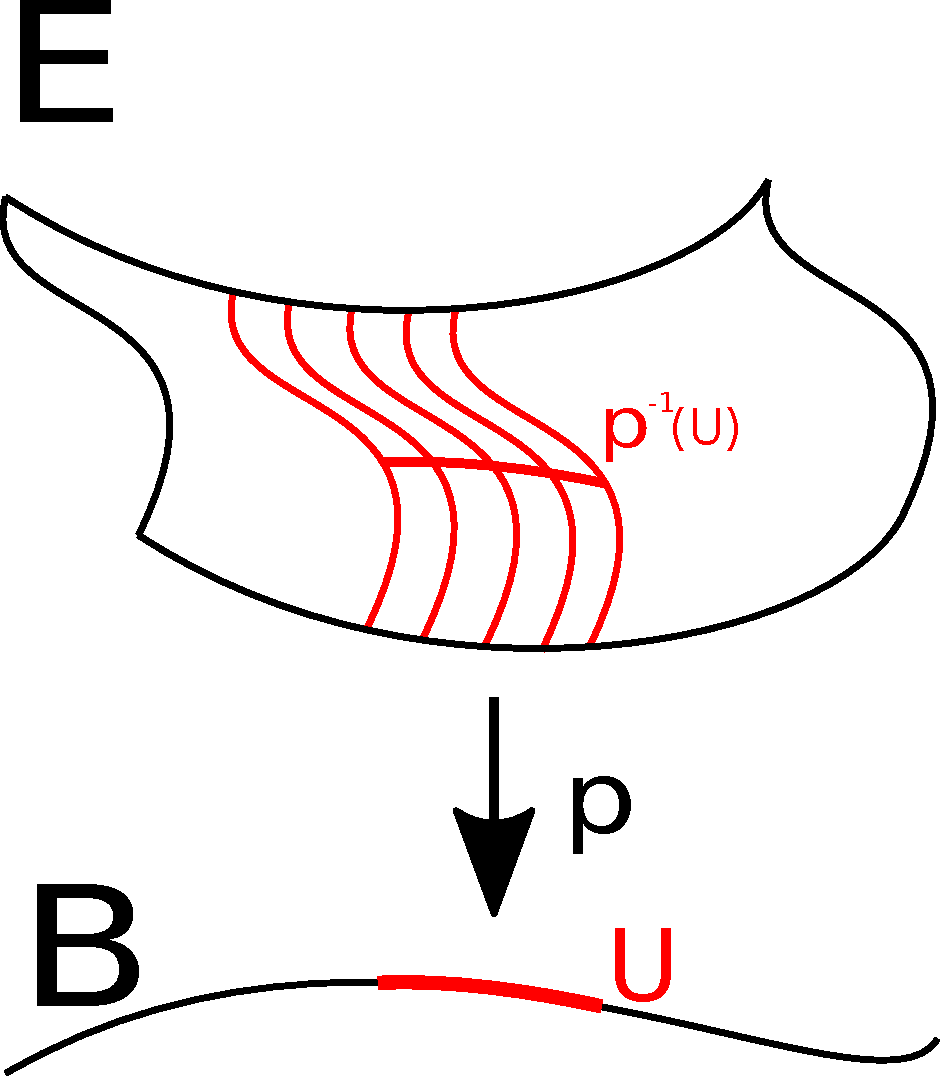
\includegraphics[scale=0.3]{fibrado.pdf}
        \caption{Illustration of the local triviality of a vector bundle.}
    \end{figure}
    
    Note that every vector bundle $\xi=(E,p,B)$ admits a section $s:B\to E$, called the zero section\index{section!zero}, defined by 
    $s(b)=0\in p^{-1}(b)$.
    
    \begin{defi}\label{fv_iso}
        We say that two $\R^{n}-$vector bundles $\xi=(E,p,B)$ and $\xi'=(E',q,B)$ are isomorphic\index{isomorphism}, denoted by 
        $\xi\cong\xi'$, if there exists a homeomorphism $h:E\to E'$ such that $q\circ h=p$ and $h|_{p^{-1}(b)}:p^{-1}(b)\to q^{-1}(b)$ is a 
        vector space isomorphism\index{isomorphism!vector space} for every $b\in B$.
    \end{defi}
    
    Now, let us recall how to specifically define the tangent and normal vector bundles of a smooth manifold and of a smooth embedding, 
    respectively.
    
    Consider $M^{m}$ a smooth $m$-dimensional manifold and define $TM=\ds\bigcup_{b\in M}\{b\}\times T_{b}M$, recalling that $T_{b}M$ is the 
    tangent space of $M$ at $b$.
    
    Thus, $\tau(M)=(TM,p_{1},M)$ defines an $\R^{m}$-vector bundle, where the fiber over $b\in M$ is $p_{1}^{-1}(b)=\{b\}\times T_{b}M$.
    
    \begin{defi}\label{defi_fvt}
        $\tau(M)$ is called the tangent vector bundle\index{bundle!vector!tangent} of the smooth manifold\index{manifold!smooth} $M$.
    \end{defi}
    
    Recall that an immersion\index{immersion} $i:N^{n}\to M^{n+k}$ is a map between smooth manifolds such that its differential 
    $d_{b}i:T_{b}N\to T_{i(b)}M$ is an injective linear transformation for every $b\in N$.

    In this context, we can ensure that $d_{b}i(T_{b}N)$ is a linear subspace of $T_{i(b)}M$. Thus, the set 
    $E(i)=\{ (b,v)\in N\times T_{i(b)}M \ : \ v\in [d_{b}i(T_{b}N)]^{\perp}\subset T_{i(b)}M \}$ is well defined.
    
    Therefore, $\nu(i)=(E(i),p_{1},N)$ is an $\R^{k}$-vector bundle, where the fiber over $b\in N$ is given by 
    $p_{1}^{-1}(b)=\{b\}\times [d_{b}i(T_{b}N)]^{\perp}$.
    
    \begin{defi}\label{defi_fvn}
        $\nu(i)$ is called the normal vector bundle\index{vector bundle!normal} of the immersion $i:N\to M$.
    \end{defi}
    
    Note that the normal vector bundle can also be defined for a smooth embedding\index{embedding!smooth}, since every smooth embedding is 
    both a topological embedding\index{embedding!topological} and an immersion\index{immersion}.
    
    To conclude the topics about vector bundles, let us present the following relation between the tangent and normal vector bundles of a 
    smooth embedding between smooth manifolds\index{manifold!smooth}, whose proof can be found in 
    (\cite{milnor_1}, Corollaries 3.4 and 3.5, pp. 30–31).
    
    \begin{teo}\label{dualidade_whitney_vet}
        If $i:N^{n}\to M^{n+k}$ is a smooth embedding between smooth manifolds, then:
        $$ \tau(N)\oplus\nu(i)\cong i^{*}(\tau(M)) $$
    \end{teo}



    \section{Fibration and Pair Fibration}\label{secao_fib_pares}

    \

    In this section, we will define the concept of pair fibration\index{fibration!of pairs}, also developed by Fadell in \cite{fadell_1}, 
    which can be considered as a fibration\index{fibration} whose total space is a pair of topological spaces.

    The definition of pair fibration will be necessary when we define generalized bundles\index{bundle!generalized} in the next section. We 
    will use the properties developed in this section as an intermediate step in the proofs of results involving generalized bundles.
    
    Except for Example \ref{pf_fv}, all the results presented throughout this section can be found, with few details, in \cite{fadell_1} and 
    \cite{brown}.
    
    \begin{defi}\label{PLH}
        We say that a map $p:E\to B$ satisfies the homotopy lifting property\index{homotopy lifting property} (HLP) over a topological space 
        $X$ if, for any maps $h:X\to E$ and $H:X\times I\to B$ such that $H(\_,0)=p\circ h$, there exists a continuous map 
        $\wt{H}:X\times I\to E$ such that $\wt{H}(\_,0)=h$ and $p\circ\wt{H}=H$. In this case, we have the following commutative diagram: 
        $$ \xymatrix @C=0.5cm {
            X\times \{ 0 \} \ar[rrr]^-{h} \ar@{^(->}[dd] &&& E \ar[dd]^-{p} \\
            &&& \\
            X\times I \ar[rrr]^-{H} \ar[rrruu]^-{\wt{H}} &&& B
        }$$
    \end{defi}

    \
    
    \begin{defi}
        A onto map $p:E\to B$ is said to be a fibration\index{fibration} if $p$ satisfies the HLP over any topological space $X$.
    
        In this context, we call the triple $\mathcal{F}=(E,p,B)$ a fibration over a base space $B$, with total space $E$ and fiber 
        $F=p^{-1}(b)$ over $b\in B$. We say that a map $s:B\to E$ is a section\index{section} of $\mathcal{F}$ if $p\circ s=1$.
    \end{defi}
    
    \begin{defi}{\bf (Pair Fibration)}\label{defi_par-fib}
        Let $p:E\to B$ be a onto map and $E_{0}\subset E$. We call $(\mathcal{F},\mathcal{F}_{0})=(E,E_{0},p,B)$ a pair 
        fibration\index{fibration!of pairs} if, for any topological space $X$ and any maps $h:X\to E$ and $H:X\times I\to B$ such that 
        $H(\_,0)=p\circ h$, there exists a continuous map $\wt{H}:X\times I\to E$ such that $\wt{H}(\_,0)=h$, $p\circ\wt{H}=H$, and if 
        $x_{0}\in X$ is such that $h(x_{0})\in E_{0}$, then $\wt{H}(x_{0},\_)\in E_{0}$.
    
        In this context, we say that $(\mathcal{F},\mathcal{F}_{0})$ is a pair fibration over a base space $B$, with total space $(E,E_{0})$ 
        and fiber $(F,F_{0})=(p^{-1}(b),p^{-1}(b)\cap E_{0})$ over $b\in B$.
    
        We also say that a map $s:B\to E$ is a section\index{section} of $(\mathcal{F},\mathcal{F}_{0})$ if $p\circ s=1$.
    \end{defi}
    
    Note that Definition \ref{defi_par-fib} guarantees that $\mathcal{F}=(E,p,B)$ and $\mathcal{F}_{0}=(E_{0},p_{0}=p_{|E_{0}},B)$ are 
    fibrations.
    
    Historically, the concept of fibration coincides with the concept of "fiber space\index{fiber space}" given by Hurewicz in 
    (\cite{hurewicz}, Section 1, p. 956), as also shown in (\cite{hurewicz}, Section 2, p. 957). Thus, the concept of pair fibration 
    coincides with the so-called "fibered pair\index{fibered pair}" given by Fadell in (\cite{fadell_1}, Definition 2.3, p. 489), as shown 
    in (\cite{brown}, Lemma 1.4, p. 183).
    
    As the simplest example of a pair fibration, we have the expected one:

    \begin{ex}\label{pf_trivial}
        Considering $B$ an arbitrary topological space, we obtain a pair fibration 
        $(\varepsilon_{B}^{n},\varepsilon_{B}^{n,0})=(B\times\R^{n},B\times(\R^{n}-\{ 0 \}),p_{1},B)$ with fiber homeomorphic to 
        $(\R^{n},\R^{n}-\{ 0 \})$.
    \end{ex}
    \begin{proof}

        \
    
        Initially, consider $X$ any topological space and maps $h:X\to B\times\R^{n}$ and $H:X\times I\to B$ such that the following 
        commutative diagram is obtained:
        $$\xymatrix @C=0.5cm {
            X\times\{ 0 \} \ar[rrr]^-{h} \ar@{^(->}[dd] &&& B\times\R^{n} \ar[dd]^-{p_{1}} \\
            &&& \\
            X\times I \ar[rrr]^-{H} &&& B
        }$$

        \
        
        Since $h=(h_{1},h_{2})$, define $\wt{H}:X\times I\to B\times\R^{n}$ by $\wt{H}(x,t)=(H(x,t),h_{2}(x))$. Clearly, $\wt{H}$ is 
        continuous, $p_{1}\circ\wt{H}=H$, and $\wt{H}(\_,0)=h$, since $H(\_,0)=h_{1}$. Furthermore, if $x_{0}\in X$ is such that 
        $h(x_{0})\in B\times (\R^{n}-\{ 0 \})$, then $h_{2}(x_{0})\in \R^{n}-\{ 0 \}$, and thus, 
        $\wt{H}(x_{0},\_)\in B\times(\R^{n}-\{ 0 \})$.
        
        Finally, given $(F,F_{0})$ the fiber of $(\mathcal{F},\mathcal{F}_{0})$ over any $b\in B$, we have:

        \
        
        $\begin{array}{rl}
            F \ = & p_{1}^{-1}(b) \\
            = & \{ b \}\times\R^{n} \\
            \approx & \R^{n}
        \end{array}$
        
        \
        
        \
        
        $\begin{array}{rl}
            F_{0} \ = & p_{1}^{-1}(b)\cap [B\times(\R^{n}-\{ 0 \})] \\
            = & [\{ b \}\times\R^{n}]\cap [B\times(\R^{n}-\{ 0 \})] \\
            = & \{ b \}\times(\R^{n}-\{ 0 \}) \\
            \approx & \R^{n}-\{ 0 \}
        \end{array}$ 

        \
        
        Thus, $(\varepsilon_{B}^{n},\varepsilon_{B}^{n,0})$ is indeed a pair fibration.
    
    \end{proof}
    
    Note that Example \ref{pf_trivial} also remains valid if we replace $\R^{n}$ with any topological space $F$ and $\R^{n}-\{ 0 \}$ with 
    any subspace $F_{0}\subset F$. However, in this case, the fiber would be homeomorphic to the pair $(F,F_{0})$.
    
    Next, we will present an alternative way of constructing pair fibrations, whose proof can be found in (\cite{allaud}, Theorem 2.5, p.241).
    
    \begin{teo}\label{teo_hurewicz}
        Let $p:E\to B$ be a onto map with $B$ paracompact, and pairs $(F,F_{0})$ and $(E,E_{0})$. If there exists an open covering 
        $\mathcal{U}$ of $B$ such that, for each $U\in\mathcal{U}$, there exists a homeomorphism 
        $h_{U}:(U\times F,U\times F_{0})\to (p^{-1}(U),p^{-1}(U)\cap E_{0})$ such that $p\circ h_{U}=p_{1}$, then $(E,E_{0},p,B)$ is a pair 
        fibration.
    \end{teo}

    Theorem \ref{teo_hurewicz} can be considered the version of the Hurewicz Uniformization Theorem\index{theorem!Hurewicz Uniformization 
    Theorem}\footnote{For more details on the Hurewicz Uniformization Theorem, see \cite{hurewicz}.} for fibrations of pairs.

    Thus, we can obtain the following:
    
    \begin{ex}\label{pf_fv}
        Every $\R^{n}$-vector bundle\index{vector bundle}, over a paracompact base, can be associated with a pair 
        fibration\index{fibration!of pairs}, whose fiber is homeomorphic to the pair $(\R^{n},\R^{n}-\{ 0 \})$.
    \end{ex}
    \begin{proof}
    
    \
    
    First, consider $\xi=(E,p,B)$ an $\R^{n}$-vector bundle over a paracompact $B$. By Definition \ref{fv_defi}, we know that there exists an 
    open cover $\mathcal{U}$ of $B$ such that, for every $U\in\mathcal{U}$, there exists a homeomorphism $h_{U}:U\times\R^{n}\to p^{-1}(U)$ 
    satisfying $p\circ h_{U}=p_{1}$.
    
    Denoting by $s:B\to E$ the zero section\index{zero section} of $\xi$ and $E_{0}=E-s(B)$, it is clear that we can consider 
    $h_{U}:(U\times\R^{n},U\times(\R^{n}-\{ 0 \}))\to (p^{-1}(U),p^{-1}(U)\cap E_{0})$ as a homeomorphism of pairs.
    
    Therefore, it follows from Theorem \ref{teo_hurewicz} that $(\xi,\xi_{0})=(E,E_{0},p,B)$ is a pair fibration.
    
    \end{proof}
    
    Now, as the final part of this section, let us see how to construct some pair fibrations from others.
    
    \begin{lem}\label{pf_restricao}
        Let $(\mathcal{F},\mathcal{F}_{0})=(E,E_{0},p,B)$ be a pair fibration and $U\subset B$ any subset. Then, 
        $(\mathcal{F},\mathcal{F}_{0})_{|U}=(p^{-1}(U),p^{-1}(U)\cap E_{0},p_{|p^{-1}(U)},U)$ will be a pair 
        fibration\index{fibration!of pairs} with fiber equal to the fiber of $(\mathcal{F},\mathcal{F}_{0})$.
    \end{lem}
    \begin{proof}
    
    \
    
    First, denote $q=p_{|p^{-1}(U)}$ and consider $X$ an arbitrary topological space and maps $h:X\to p^{-1}(U)$ and $H:X\times I\to U$ such 
    that the following diagram commutes:
    $$ \xymatrix @C=0.5cm {
        X\times\{ 0 \} \ar[rrr]^-{h} \ar@{^(->}[dd] &&& p^{-1}(U) \ar[dd]^-{q} \\
        &&& \\
        X\times I \ar[rrr]^-{H} &&& U 
    }$$
    
    Since $Im(H)\subset U\subset B$ and $(\mathcal{F},\mathcal{F}_{0})$ is a pair fibration, there exists a map $\wt{H}:X\times I\to E$ such 
    that $p\circ\wt{H}=H$ and $\wt{H}(\_,0)=h$. On the other hand, $Im(p\circ\wt{H})=Im(H)\subset U$, and thus $Im(\wt{H})\subset p^{-1}(U)$.
    
    Moreover, if $x_{0}\in X$ is such that $h(x_{0})\in E_{0}$, then $\wt{H}(x_{0},\_)\in E_{0}$. That is, if 
    $h(x_{0})\in p^{-1}(U)\cap E_{0}$, then $\wt{H}(x_{0},\_)\in p^{-1}(U)\cap E_{0}$.
    
    Finally, letting $(F',F'_{0})$ and $(F,F_{0})$ be the fibers of $(\mathcal{F},\mathcal{F}_{0})_{|U}$ and $(\mathcal{F},\mathcal{F}_{0})$, 
    respectively, over the same $b\in U$, we have:

    \
    
    $\begin{array}{rl}
        F' \ = & q^{-1}(b) \\
        = & p^{-1}(b)\cap p^{-1}(U) \\
        = & p^{-1}(b) \\
        = & F
    \end{array}$

    \

    \

    $\begin{array}{rl}
        F'_{0} \ = & q^{-1}(b)\bigcap [p^{-1}(U)\cap E_{0}] \\
        = & p^{-1}(b)\bigcap [p^{-1}(U)\cap E_{0}] \\
        = & p^{-1}(b)\cap E_{0} \\
        = & F_{0}
    \end{array}$

    \
    
    Therefore, $(\mathcal{F},\mathcal{F}_{0})_{|U}$ is a pair fibration.
    
    \end{proof}

    \begin{lem}\label{pf_pullback}
        Let $(\mathcal{F},\mathcal{F}_{0})=(E,E_{0},p,B)$ be a pair fibration and $f:B'\to B$ a map. Then, 
        $f^{*}(\mathcal{F},\mathcal{F}_{0})=(f^{*}E,f^{*}E_{0},p_{1},B')$ is also a pair fibration\index{fibration!of pairs} with fiber 
        homeomorphic to the fiber of $(\mathcal{F},\mathcal{F}_{0})$, where:
        
        \begin{enumerate}
            \item $f^{*}E=\{ (b',e)\in B'\times E \ : \ f(b')=p(e) \}$
            \item $f^{*}E_{0}=\{ (b',e)\in f^{*}E \ : \ e\in E_{0} \}$
        \end{enumerate}
    \end{lem}
    
    \begin{proof}
    
    \

        At first, let $X$ be any topological space and $h:X\to f^{*}E$ and $H:X\times I\to B'$ maps such that the following diagram commutes:
        $$\xymatrix @C=0.5cm {
            X\times\{ 0 \} \ar[rrr]^-{h} \ar@{^(->}[dd] &&& f^{*}E \ar[rrr]^-{p_{2}} \ar[dd]^-{p_{1}} &&& E \ar[dd]^-{p} \\
            &&& &&& \\
            X\times I \ar[rrr]^-{H} &&& B' \ar[rrr]^-{f} &&& B
        }$$

        \
        
        Denoting $g=p_{2}\circ h:X\to E$ and $G=f\circ H:X\times I\to B$, since the diagram above commutes and 
        $(\mathcal{F},\mathcal{F}_{0})$ is a pair fibration, there exists $\widetilde{G}:X\times I\to E$ such that 
        $p\circ\widetilde{G}=G$, $\widetilde{G}(\_,0)=g$, and if $x_{0}\in X$ is such that $g(x_{0})\in E_{0}$, then 
        $\widetilde{G}(x_{0},\_)\in E_{0}$.
        
        On the other hand, it is clear that $\widetilde{H}=(H,\widetilde{G}):X\times I\to f^{*}E$ is well-defined, since 
        $f\circ H=G=p\circ\widetilde{G}$. Moreover, $p_{1}\circ\widetilde{H}=H$ and $\widetilde{H}(\_,0)=h$, since $H(\_,0)=p_{1}\circ h$ 
        and $\widetilde{G}(\_,0)=p_{2}\circ h$.
        
        Thus, if $x_{0}\in X$ is such that $h(x_{0})\in f^{*}E_{0}$, then $g(x_{0})=p_{2}\circ h(x_{0})\in E_{0}$, and consequently, 
        $\widetilde{G}(x_{0},\_)\in E_{0}$. Therefore, $\widetilde{H}(x_{0},\_)\in f^{*}E_{0}$.
        
        Finally, if $(F',F'_{0})$ and $(F,F_{0})$ are fibers of $f^{*}(\mathcal{F},\mathcal{F}_{0})$ and $(\mathcal{F},\mathcal{F}_{0})$ 
        over $b'_{0}\in B'$ and $f(b'_{0})\in B$, respectively, then:

        \
        
        $\begin{array}{rl}
            F' = & p_{1}^{-1}(b'_{0}) \\
            = & \{ (b',e)\in f^{*}E \ : \ b'=p_{1}(b',e)=b'_{0} \} \\
            = & \{ (b'_{0},e)\in B'\times E \ : \ f(b'_{0})=p(e) \} \\
            = & \{ (b'_{0},e)\in B'\times E \ : \ e\in p^{-1}(f(b'_{0})) \} \\
            = & \{ b'_{0} \}\times p^{-1}(f(b'_{0})) \\
            = & \{ b'_{0} \}\times F \\
            \approx & F
        \end{array}$
        
        \

        \
        
        $\begin{array}{rl}
            F'_{0} = & p_{1}^{-1}(b'_{0})\cap f^{*}E_{0} \\
            = & (\{ b'_{0} \}\times F)\cap f^{*}E_{0} \\
            = & \{ b'_{0} \}\times (F\cap E_{0}) \\
            = & \{ b'_{0} \}\times F_{0} \\
            \approx & F_{0}
        \end{array}$
        
        \
        
        Therefore, $f^{*}(\mathcal{F},\mathcal{F}_{0})$ is indeed a pair fibration.
    \end{proof}

    \begin{lem}\label{pf_produto}
        Let $(\mathcal{F},\mathcal{F}_{0})=(E,E_{0},p,B)$ and $(\mathcal{F'},\mathcal{F'}_{0})=(E',E'_{0},q,B')$ be two pair fibrations. 
        Then, $(\mathcal{F},\mathcal{F}_{0})\times(\mathcal{F'},\mathcal{F'}_{0})=(E'',E''_{0},r,B'')$ will be a pair 
        fibration\index{fibration!of pairs} with fiber equal to the product of the fibers of $(\mathcal{F},\mathcal{F}_{0})$ and 
        $(\mathcal{F'},\mathcal{F'}_{0})$, where:
        
        \begin{enumerate}
            \item $E''=E\times E'$
            \item $E''_{0}=(E\times E'_{0})\cup (E_{0}\times E')$
            \item $r=p\times q$
        \end{enumerate}
        
    \end{lem}
    
    \begin{proof}
    
    \
    
        At first, let $X$ be any topological space and $h:X\to E''$ and $H:X\times I\to B''$ maps such that the following diagram commutes:
        $$\xymatrix @C=0.5cm {
            X\times\{ 0 \} \ar[rrr]^-{h} \ar@{^(->}[dd] &&& E'' \ar[dd]^-{r} \\
            &&& &&& \\
            X\times I \ar[rrr]^-{H} &&& B'' 
        }$$

        \
        
        Since $h=(h_{1},h_{2})$, $H=(H_{1},H_{2})$, and $H(\_,0)=r\circ h$, we have that $H_{1}(\_,0)=p\circ h_{1}$ and 
        $H_{2}(\_,0)=q\circ h_{2}$. As $(\mathcal{F},\mathcal{F}_{0})$ and $(\mathcal{F'},\mathcal{F'}_{0})$ are pair fibrations, there 
        exist maps $\wt{H_{1}}:X\times I\to E$ and $\wt{H_{2}}:X\times I\to E'$ such that $p\circ\wt{H_{1}}=H_{1}$, $q\circ\wt{H_{2}}=H_{2}$, 
        $\wt{H_{1}}(\_,0)=h_{1}$, $\wt{H_{2}}(\_,0)=h_{2}$, and if $x_{0}\in X$ is such that $h_{1}(x_{0})\in E_{0}$, then 
        $\wt{H_{1}}(x_{0},\_)\in E_{0}$. Moreover, if $x_{0}\in X$ is such that $h_{2}(x_{0})\in E'_{0}$, then 
        $\wt{H_{2}}(x_{0},\_)\in E'_{0}$.
        
        Thus, defining $\wt{H}=(\wt{H_{1}},\wt{H_{2}}):X\times I\to E''$, it is clear that $\wt{H}(\_,0)=h$ and $r\circ\wt{H}=H$. 
        Furthermore, if $x_{0}\in X$ is such that $h(x_{0})\in E''_{0}$, then $h_{1}(x_{0})\in E_{0}$ or $h_{2}(x_{0})\in E'_{0}$. 
        Hence, $\wt{H_{1}}(x_{0},\_)\in E_{0}$ or $\wt{H_{2}}(x_{0},\_)\in E'_{0}$, that is, $\wt{H}(x_{0},\_)\in E''_{0}$.
        
        Finally, consider, respectively, $(F,F_{0})$, $(F',F'_{0})$, and $(F'',F''_{0})$ the fibers of 
        $(\mathcal{F},\mathcal{F}_{0})$, $(\mathcal{F'},\mathcal{F'}_{0})$, and 
        $(\mathcal{F},\mathcal{F}_{0})\times (\mathcal{F'},\mathcal{F'}_{0})$ over $b\in B$, $b'\in B'$, and $(b,b')\in B''$. Then:

        \
        
        $\begin{array}{rl}
            F'' \ = & r^{-1}(b,b') \\
            = & p^{-1}(b)\times q^{-1}(b') \\
            = & F\times F'
        \end{array}$
        
        \

        \

        $\begin{array}{rl}
            F''_{0} \ = & r^{-1}(b,b')\cap E''_{0} \\
            = & (F\times F')\bigcap [(E\times E'_{0})\cup (E_{0}\times E')] \\
            = & [(F\times F')\cap (E\times E'_{0})]\bigcup [(F\times F')\cap (E_{0}\times E')] \\
            = & [F\times (F'\cap E'_{0})]\bigcup [(F\cap E_{0})\times F'] \\
            = & (F\times F'_{0})\cup (F_{0}\times F')
        \end{array}$
        
        \
        
        Therefore, $(\mathcal{F},\mathcal{F}_{0})\times (\mathcal{F'},\mathcal{F'}_{0})$ will be a pair fibration.
        
    \end{proof}

    

    \section{Generalized Bundle}\label{secao_fib_gener}

    \

    In this section, we will present the tool developed by Fadell in \cite{fadell_1} that allows us to generalize 
    tangent\index{vector bundle!tangent} and normal\index{vector bundle!normal} vector bundles of smooth manifolds\index{manifold!smooth} to 
    topological manifolds\index{manifold!topological}. This tool is called the generalized bundle.

    Except for examples \ref{fht_sobre_ponto} and \ref{fht_fv}, lemmas \ref{iso_homot} and \ref{iso_homot_2}, and propositions 
    \ref{iso_fv_fht}, \ref{iso_homeo}, \ref{fht_tang_cart}, and \ref{iso_merg_lf_2}, all other results were taken from \cite{fadell_1}. 
    However, we will provide more detailed proofs of these results here.
    
    \begin{defi}{\bf (Generalized Bundle)}\label{defi_fib_gen}
        A pair fibration\index{pair fibration} $(\mathcal{F},\mathcal{F}_{0})=(E,E_{0},p,B)$ is said to be an $\R^{n}$-generalized 
        bundle\index{generalized bundle} if:
    
        \begin{enumerate}
            \item There exists a section\index{section} $s:B\to E$ of $(\mathcal{F},\mathcal{F}_{0})$ such that $E_{0}$ is realized, i.e., 
            $E_{0}=E-s(B)$.
            \item Every fiber $(F,F_{0})$ of $(\mathcal{F},\mathcal{F}_{0})$ satisfies $(F,F_{0})\sim (\R^{n},\R^{n}-\{ 0 \})$.
        \end{enumerate}
    \end{defi}
    
    \begin{ex}\label{fht_trivial}
        The pair fibration $(\varepsilon^{n}_{B},\varepsilon^{n,0}_{B})$ is an $\R^{n}-$generalized bundle.
    \end{ex}
    \begin{proof}
        
        \
    
        Since Example \ref{pf_trivial} already shows that $(\varepsilon^{n}_{B},\varepsilon^{n,0}_{B})$ is a pair fibration with a fiber 
        homeomorphic to the pair $(\R^{n},\R^{n}-\{ 0 \})$, it is enough to define a section of $(\varepsilon^{n}_{B},\varepsilon^{n,0}_{B})$ 
        that realizes $B\times(\R^{n}-\{ 0 \})$.
    
        Note that $s:B\to B\times\R^{n}$ defined by $s(b)=(b,0)$ is the required section.
    
        Therefore, $(\varepsilon^{n}_{B},\varepsilon^{n,0}_{B})$ is an $\R^{n}-$generalized bundle.
    
    \end{proof}
    
    \begin{lem}\label{fht_restricao}
        If $(\mathcal{F},\mathcal{F}_{0})$ is an $\R^{n}-$generalized bundle\index{generalized bundle} over $B$, then 
        $(\mathcal{F},\mathcal{F}_{0})_{|U}$ will also be an $\R^{n}-$generalized bundle for any $U\subset B$.
    \end{lem}
    \begin{proof}
        
        \
    
        From Lemma \ref{pf_restricao}, we already know that if $(\mathcal{F},\mathcal{F}_{0})$ is a pair fibration\index{pair fibration}, 
        then for any arbitrary $U\subset B$, $(\mathcal{F},\mathcal{F}_{0})_{|U}$ will also be a pair fibration with fiber equal to the fiber 
        of $(\mathcal{F},\mathcal{F}_{0})$.
        
        Thus, let $(\mathcal{F},\mathcal{F}_{0})=(E,E_{0},p,B)$ and 
        $(\mathcal{F},\mathcal{F}_{0})_{|U}=(p^{-1}(U),p^{-1}(U)\cap E_{0},p_{|p^{-1}(U)},U)$. It is enough to find a 
        section\index{section} of $(\mathcal{F},\mathcal{F}_{0})_{|U}$ that realizes $p^{-1}(U)\cap E_{0}$.
    
        Since $(\mathcal{F},\mathcal{F}_{0})$ is an $\R^{n}-$generalized bundle, there exists a section $s:B\to E$ of 
        $(\mathcal{F},\mathcal{F}_{0})$ that realizes $E_{0}$.
        
        Now, define $s'=s_{|U}:U\to p^{-1}(U)$. Clearly, $Im(s')\subset p^{-1}(U)$ because $p\circ s(U)=U$. Furthermore, we have:

        \
    
        $\begin{array}{rl}
            p^{-1}(U)\cap E_{0} = & p^{-1}(U)\bigcap [E-s(B)] \\
            = & [p^{-1}(U)\cap E]-[p^{-1}(U)\cap s(B)] \\
            = & p^{-1}(U)-s(U) \\
            = & p^{-1}(U)-s'(U)
        \end{array}$

        \
    
        Therefore, $(\mathcal{F},\mathcal{F}_{0})_{|U}$ will also be an $\R^{n}-$generalized bundle for all $U\subset B$.
    
    \end{proof}
    
    Following the notation of Lemma \ref{fht_restricao}, if $(\mathcal{F},\mathcal{F}_{0})$ is an $\R^{n}-$generalized bundle, we call 
    $(\mathcal{F},\mathcal{F}_{0})_{|U}$ the restriction of the $\R^{n}-$generalized bundle\index{generalized bundle!restriction} of 
    $(\mathcal{F},\mathcal{F}_{0})$ to $U\subset B$.
    
    \begin{defi}
        Let $(\mathcal{F},\mathcal{F}_{0})=(E,E_{0},p,B)$ and $(\mathcal{F'},\mathcal{F'}_{0})=(E',E'_{0},q,B)$ be $\R^{n}$-generalized 
        bundles over the same base. We call $\phi:(\mathcal{F},\mathcal{F}_{0})\to (\mathcal{F'},\mathcal{F'}_{0})$ a fiber 
        map\index{fiber map} if $\phi:(E,E_{0})\to (E',E'_{0})$ is a map that preserves the fibers, i.e., $q\circ\phi=p$.
    \end{defi}

    \begin{defi}\label{defi_iso_homot}
        We say that two $\R^{n}-$generalized bundles over the same base, $(\mathcal{F},\mathcal{F}_{0})=(E,E_{0},p,B)$ and 
        $(\mathcal{F'},\mathcal{F'}_{0})=(E',E'_{0},q,B)$, are homotopically isomorphic if there exist fiber maps 
        $\phi:(\mathcal{F},\mathcal{F}_{0})\rightleftarrows (\mathcal{F'},\mathcal{F'}_{0}):\psi$ and $H:(E,E_{0})\times I\to (E,E_{0})$ and 
        $G:(E',E'_{0})\times I\to (E',E'_{0})$ homotopies such that:
        
        \

        $\begin{array}{lcccl}
            1. \ H(\_,0)=\psi\circ\phi            & & & & 4. \ G(\_,0)=\phi\circ\psi \\
            2. \ H(\_,1)=1                        & & & & 5. \ G(\_,1)=1 \\
            3. \ p\circ H(\_,t)=p, \forall t\in I & & & & 6. \ q\circ G(\_,t)=q, \forall t\in I
        \end{array}$

        \
    
        The homotopy isomorphism\index{isomorphism!homotopy}, defined above, will be denoted by 
        $(\mathcal{F},\mathcal{F}_{0})\sim_{f} (\mathcal{F'},\mathcal{F'}_{0})$.
    \end{defi}
    
        The notion of homotopy isomorphism, as given in the definition above, coincides with the concept of "fiber homotopy 
        equivalence\index{fiber homotopy equivalence}" given by Fadell in (\cite{fadell_1}, Definition 2.4, p. 489).
    
    \begin{defi}
        We call a $\R^{n}-$generalized bundle $(\mathcal{F},\mathcal{F}_{0})$, over $B$, locally trivial\index{locally trivial} if there 
        exists an open cover $\mathcal{U}$ of $B$ such that 
        $(\mathcal{F},\mathcal{F}_{0})_{|U}\sim_{f} (\varepsilon^{n}_{U},\varepsilon^{n,0}_{U})$, for every $U\in\mathcal{U}$. In particular, 
        $(\mathcal{F},\mathcal{F}_{0})$ will be called a trivial $\R^{n}-$generalized bundle\index{fiber bundle!generalized!trivial} if 
        $(\mathcal{F},\mathcal{F}_{0})\sim_{f} (\varepsilon^{n}_{B},\varepsilon^{n,0}_{B})$.
    \end{defi}
    
    \begin{ex}\label{fht_sobre_ponto}
        Every $\R^{n}-$generalized bundle over a point is trivial.
    \end{ex}
    \begin{proof}
    
        \
    
        Let us denote by $(\mathcal{F},\mathcal{F}_{0})=(E,E_{0},p,\{ * \})$ a $\R^{n}-$generalized bundle whose base space consists of only 
        one point.
    
        Thus, it is clear that $(E,E_{0})=(p^{-1}(*),p^{-1}(*)\cap E_{0})\sim (\R^{n},\R^{n}-\{0 \})$, that is, there exist fiber maps 
        $\phi:(E,E_{0})\rightleftarrows (\R^{n},\R^{n}-\{ 0 \}):\psi$ and homotopies $H:(E,E_{0})\times I\to (E,E_{0})$ and 
        $G:(\R^{n},\R^{n}-\{0 \})\times I\to (\R^{n},\R^{n}-\{0 \})$ such that $H(\_,0)=\psi\circ\phi$, $H(\_,1)=1$, $G(\_,0)=\phi\circ\psi$ 
        and $G(\_,1)=1$.
    
        Thus, the following fiber maps\index{fiber map} and homotopies are well-defined:
    
        \begin{enumerate}
            \item $\overline{\phi}:(E,E_{0})\rightleftarrows (\{ * \}\times\R^{n},\{ * \}\times\R^{n}-\{0 \}):\overline{\psi}$ \\
            $ \overline{\phi}(e)=(*,\phi(e)) $ \\
            $ \overline{\psi}(*,x)=\psi(x) $
            \item $\overline{H}:(E,E_{0})\times I\to (E,E_{0})$ \\
            $ \overline{H}(e,t)=H(e,t) $
            \item $\overline{G}:(\{ * \}\times\R^{n},\{ * \}\times\R^{n}-\{0 \})\times I \to (\{ * \}\times\R^{n},\{ * \}\times\R^{n}-\{0 \})$ \\
            $ \overline{G}((*,x),t)=(*,G(x,t)) $
        \end{enumerate}
    
        It is clear that $\overline{H}(\_,1)=1$, $\overline{G}(\_,1)=1$, $p\circ\overline{H}(\_,t)=p$ and $p_{1}\circ\overline{G}(\_,t)=p_{1}$ 
        for any $t\in I$. Also:

        \
    
        $\begin{array}{rl}
            \forall e\in E, \ \overline{H}(e,0) \ = & H(e,0) \\
            = & \psi\circ\phi(e) \\
            = & \overline{\psi}(*,\phi(e)) \\
            = & \overline{\psi}\circ\overline{\phi}(e)
        \end{array}$

        \

        \

        $\begin{array}{rl}
            \forall x\in \R^{n}, \ \overline{G}((*,x),0) \ = & (*,G(x,0)) \\
            = & (*,\phi\circ\psi(x)) \\
            = & \overline{\phi}(\psi(x)) \\
            = & \overline{\phi}\circ\overline{\psi}(*,x)
        \end{array}$

        \
    
        Therefore, $(\mathcal{F},\mathcal{F}_{0})\sim_{f}(\varepsilon^{n}_{\{ * \}},\varepsilon^{n,0}_{\{ * \}})$.
    
    \end{proof}

    Regarding specific conditions, the homotopy isomorphism\index{isomorphism!homotopy} can be guaranteed more simply, as follows:

    \begin{lem}\label{iso_homot}
        Let $(\mathcal{F},\mathcal{F}_{0})$ and $(\mathcal{F'},\mathcal{F'}_{0})$ be two $\R^{n}-$generalized bundles, over the same base. 
        If $\phi:(\mathcal{F},\mathcal{F}_{0})\to (\mathcal{F'},\mathcal{F'}_{0})$ is a fiber map\index{map!fiber} such that $\phi$ is a 
        homeomorphism, then $(\mathcal{F},\mathcal{F}_{0})\sim_{f} (\mathcal{F'},\mathcal{F'}_{0})$.
    \end{lem}
    \begin{proof}
    
        \
        
        Initially, since $\phi$ is a homeomorphism and $q\circ\phi=p$, it follows that $p\circ\phi^{-1}=q$, that is, 
        $\phi^{-1}:(\mathcal{F},\mathcal{F}_{0})\to (\mathcal{F'},\mathcal{F'}_{0})$ is also a fiber map.
        
        Thus, it is evident that $(\mathcal{F},\mathcal{F}_{0})\sim_{f} (\mathcal{F},\mathcal{F}_{0})$, since it is sufficient to define 
        trivial homotopies for the conditions of homotopy isomorphism to be satisfied.
        
    \end{proof}
    
    In this way, using Lemma \ref{iso_homot} and the construction from Example \ref{pf_fv}, we obtain the following:
    
    \begin{ex}\label{fht_fv}
        If $\xi$ is an $\R^{n}-$vector bundle\index{bundle!vector} over a paracompact base, then its associated pair 
        fibration\index{fibration!pair} $(\xi,\xi_{0})$ will be a locally trivial $\R^{n}-$generalized bundle\index{bundle!generalized}.
    \end{ex}
    
    Therefore, we can consider that the notion of generalized bundles generalizes the concept of vector bundles. Thus, it is expected 
    that the isomorphism structure between vector bundles is preserved when passing to homotopy isomorphism\index{isomorphism!homotopy}, as 
    in the following:
    
    \begin{prop}\label{iso_fv_fht}
        Let $\xi$ and $\eta$ be two isomorphic $\R^{n}-$vector bundles\index{bundle!vector} over the same paracompact base. Then, their 
        respective associated $\R^{n}-$generalized bundles $(\xi,\xi_{0})$ and $(\eta,\eta_{0})$ are homotopy isomorphic.
    \end{prop}
    \begin{proof}
    
        \

        First, let $\xi=(E,p,B)\cong\eta=(E',q,B)$. Thus, by definition \ref{fv_iso}, there exists a homeomorphism $h:E\to E'$ such that 
        $q\circ h=p$ and $h_{|F}:F\to F'$ is a vector isomorphism\index{isomorphism!vector}, for any fibers $F$ and $F'$ of $\xi$ and $\eta$, 
        respectively, over the same $b\in B$.
        
        Let $s:B\to E$ and $s':B\to E'$ be the zero sections\index{section!zero} of $\xi$ and $\eta$, respectively, and consider 
        $E_{0}=E-s(B)$ and $E'_{0}=E'-s'(B)$. If we show that $h(E_{0})\subset E'_{0}$, then $h:(E,E_{0})\to (E',E'_{0})$ will be a 
        homeomorphism and a fiber map\index{map!fiber}, and thus, Lemma \ref{iso_homot} will guarantee that 
        $(\xi,\xi_{0})\sim_{f} (\eta,\eta_{0})$.
        
        To this end, note that:

        \
        
        $\begin{array}{rl}
            e\in E_{0} \Longrightarrow & e\in F=p^{-1}(p(e))\cong\R^{n} \text{ and } e\neq 0 \\
            \Longrightarrow & h(e)\in F'=q^{-1}(p(e))\cong\R^{n} \text{ and } h(e)\neq 0 \\
            \Longrightarrow & h(e)\in E'_{0}
        \end{array}$

        \
        
        Therefore, we conclude that $(\xi,\xi_{0})\sim_{f} (\eta,\eta_{0})$.
        
    \end{proof}
    
    \begin{lem}\label{fht_pullback}
        If $(\mathcal{F},\mathcal{F}_{0})$ is a $\R^{n}-$generalized bundle\index{bundle!generalized!trivial} over $B$ and $f:B'\to B$ is any 
        map, then $f^{*}(\mathcal{F},\mathcal{F}_{0})$ will also be a $\R^{n}-$generalized bundle. In particular, if 
        $(\mathcal{F},\mathcal{F}_{0})$ is trivial, then $f^{*}(\mathcal{F},\mathcal{F}_{0})$ will also be trivial.
    \end{lem}

    \begin{proof}

        \

        Due to lemma \ref{pf_pullback}, we already know that if $(\mathcal{F},\mathcal{F}_{0})$ is a pair fibration, then 
        $f^{*}(\mathcal{F},\mathcal{F}_{0})$ will be a pair fibration with fiber homeomorphic to the fiber of $(\mathcal{F},\mathcal{F}_{0})$. 
        Thus, denoting $(\mathcal{F},\mathcal{F}_{0})=(E,E_{0},p,B)$ and $f^{*}(\mathcal{F},\mathcal{F}_{0})=(f^{*}E,f^{*}E_{0},p_{1},B')$, 
        it is enough to show that there exists a section of $f^{*}(\mathcal{F},\mathcal{F}_{0})$ that realizes $f^{*}E_{0}$.
    
        To this end, since $(\mathcal{F},\mathcal{F}_{0})$ is a $\R^{n}-$generalized bundle, there exists a section $s:B\to E$ of 
        $(\mathcal{F},\mathcal{F}_{0})$ that realizes $E_{0}$. In this way, the section 
        $s':B'\to f^{*}E$ of $f^{*}(\mathcal{F},\mathcal{F}_{0})$ is well-defined, given by $s'(b')=(b',s(f(b')))$. Finally:

        \
        
        $\begin{array}{rl}
            f^{*}E_{0} \ = & [B'\times E_{0}]\bigcap f^{*}E \\
            = & [B'\times (E-s(B))]\bigcap f^{*}E \\
            = & [(B'\times E)-(B'\times s(B))]\bigcap f^{*}E \\
            = & [(B'\times E)\cap f^{*}E]-[(B'\times s(B))\cap f^{*}E] \\
            = & f^{*}E - \{ (b',s(b))\in B'\times s(B) \ : \ f(b')=p(s(b))=b \} \\
            = & f^{*}E - [B'\times s(f(B'))] \\
            = & f^{*}E - s'(B')
        \end{array}$
        
        \
    
        Therefore, $f^{*}(\mathcal{F},\mathcal{F}_{0})$ will be a $\R^{n}-$generalized bundle.
    
        Now, we need to show that if $(\mathcal{F},\mathcal{F}_{0})\sim_{f}(\varepsilon_{B}^{n},\varepsilon_{B}^{n,0})$, then 
        $f^{*}(\mathcal{F},\mathcal{F}_{0})\sim_{f}(\varepsilon_{B'}^{n},\varepsilon_{B'}^{n,0})$. So, suppose there exist the following 
        fiber maps and homotopies satisfying the relations below:
    
        \begin{enumerate}
            \item $\phi:(E,E_{0})\rightleftarrows(B\times \R^{n},B\times (\R^{n}-\{ 0 \})):\psi$
            \item $H:(E,E_{0})\times I\to (E,E_{0})$
            \item $G:(B\times\R^{n},B\times(\R^{n}-\{ 0 \}))\times I\to (B\times\R^{n},B\times(\R^{n}-\{ 0 \}))$
            \item $\phi$, $\psi$, $H$, and $G$ satisfy:
            
                $\begin{array}{lcccl}
                    H(\_,0)=\psi\circ\phi            & & & & G(\_,0)=\phi\circ\psi \\
                    H(\_,1)=1                        & & & & G(\_,1)=1 \\
                    p\circ H(\_,t)=p, \forall t\in I & & & & p_{1}\circ G(\_,t)=p_{1}, \forall t\in I
                \end{array}$
        \end{enumerate}

        \
    
        In this way, the following fiber maps and homotopies are well-defined:
    
        \begin{enumerate}
            \item $\overline{\phi}:(f^{*}E,f^{*}E_{0})\rightleftarrows (B'\times \R^{n},B'\times (\R^{n}-\{ 0 \})):\overline{\psi}$ \\
            $ \overline{\phi}(b',e)=(b',p_{2}\circ\phi(e)) $ \\
            $ \overline{\psi}(b',x)=(b',\psi(f(b'),x)) $
            \item $\overline{H}:(f^{*}E,f^{*}E_{0})\times I\to (f^{*}E,f^{*}E_{0})$ \\
            $ \overline{H}((b',e),t)=(b',H(e,t)) $
            \item $\overline{G}:(B'\times \R^{n},B'\times (\R^{n}-\{ 0 \}))\times I\to (B'\times \R^{n},B'\times (\R^{n}-\{ 0 \}))$ \\
            $ \overline{G}((b',x),t)=(b',p_{2}\circ G((f(b'),x),t)) $
        \end{enumerate}

        \
    
        Let's show that $\overline{\phi}$, $\overline{\psi}$, $\overline{H}$, and $\overline{G}$ satisfy the conditions of definition 
        \ref{defi_iso_homot}. Indeed:
    
        \begin{enumerate}
            \item It is clear that $p_{1}\circ\overline{H}((\_,\_),t)=p_{1}$ and $p_{1}\circ\overline{G}((\_,\_),t)=p_{1}$ for all $t\in I$
            \item It is also clear that $\overline{H}((\_,\_),1)=1$ and $\overline{G}((\_,\_),1)=1$
            \item $\forall (b',e)\in f^{*}E$, \\
                   
                    $\begin{array}{rl}
                        \overline{H}((b',e),0) \ = & (b',H(e,0)) \\
                        = & (b',\psi\circ\phi(e)) \\
                        = & (b',\psi(p_{1}\circ\phi(e),p_{2}\circ\phi(e))) \\
                        = & (b',\psi(p(e),p_{2}\circ\phi(e))) \\
                        = & (b',\psi(f(b'),p_{2}\circ\phi(e))) \\
                        = & \overline{\psi}(b',p_{2}\circ\phi(e)) \\
                        = & \overline{\psi}\circ\overline{\phi}(b',e)
                    \end{array}$
            \item $\forall (b',x)\in B'\times\R^{n}$, \\
                    
                    $\begin{array}{rl}
                        \overline{G}((b',x),0) \ = & (b',p_{2}\circ G((f(b'),x),0)) \\
                        = & (b',p_{2}\circ\phi\circ\psi(f(b'),x)) \\
                        = & \overline{\phi}(b',\psi(f(b'),x)) \\
                        = & \overline{\phi}\circ\overline{\psi}(b',x)
                    \end{array}$
        \end{enumerate}
    
        \par Therefore, $f^{*}(\mathcal{F},\mathcal{F}_{0})\sim_{f}(\varepsilon_{B'}^{n},\varepsilon_{B'}^{n,0})$.
    
    \end{proof}

    Following the notation of Lemma \ref{fht_pullback}, given $(\mathcal{F},\mathcal{F}_{0})$ a $\R^{n}-$generalized bundle, we call 
    $f^{*}(\mathcal{F},\mathcal{F}_{0})$ the $\R^{n}-$generalized bundle pullback\index{fibration!generalized!pullback} of 
    $(\mathcal{F},\mathcal{F}_{0})$ by the map $f$.

    Now, let's look at some examples involving generalized fibration pullbacks.
    
    \begin{ex}\label{fht_pullback_ex1}
    Let $(\mathcal{F},\mathcal{F}_{0})$ and $(\mathcal{F'},\mathcal{F'}_{0})$ be two $\R^{n}-$generalized bundles, over the same base $B$, 
    such that $(\mathcal{F},\mathcal{F}_{0})\sim_{f} (\mathcal{F'},\mathcal{F'}_{0})$. Then, let $1:B\to B$ be the identity map, and we have 
    $(\mathcal{F},\mathcal{F}_{0})\sim_{f} 1^{*}(\mathcal{F'},\mathcal{F'}_{0})$.
    \end{ex}
    \begin{proof}

        \

        Initially, let us denote $(\mathcal{F},\mathcal{F}_{0})=(E,E_{0},p,B)$ and $(\mathcal{F'},\mathcal{F'}_{0})=(E',E'_{0},q,B)$. Since 
        $(\mathcal{F},\mathcal{F}_{0})\sim_{f} (\mathcal{F'},\mathcal{F'}_{0})$, there exist the following fiber maps and homotopies 
        satisfying the following relations:
        
        \begin{enumerate}
            \item $\phi:(E,E_{0}) \rightleftarrows (E',E'_{0}):\psi$
            \item $H:(E,E_{0}) \times I \to (E,E_{0})$
            \item $G:(E',E'_{0}) \times I \to (E',E'_{0})$
            \item $\phi$, $\psi$, $H$, and $G$ satisfy the following relations:
            
                $\begin{array}{lccl}
                    H(\_, 0) = \psi \circ \phi & & & G(\_, 0) = \phi \circ \psi \\
                    H(\_, 1) = 1 & & & G(\_, 1) = 1 \\
                    p \circ H(\_, t) = p, \ \forall t \in I & & & q \circ G(\_, t) = q, \ \forall t \in I
                \end{array}$
        \end{enumerate}
        
        \
        
        Recall that the $\R^{n}-$generalized bundle pullback\index{fibration!generalized!pullback} 
        $1^{*}(\mathcal{F'},\mathcal{F'}_{0})=(1^{*}E',1^{*}E'_{0},p_{1},B)$ is such that:
        $$1^{*}E'=\{ (b,e')\in B\times E' : b=q(e') \}$$
        $$1^{*}E'_{0}=\{ (b,e')\in 1^{*}E' : e'\in E'_{0} \}$$
        
        \

        So, the following fiber maps\index{map!fibration} and homotopies are 
        well-defined:
        
        \begin{enumerate}
            \item $\overline{\phi}:(E,E_{0})\rightleftarrows (1^{*}E',1^{*}E'_{0}):\overline{\psi}$ \\
            $\overline{\phi}(e)=(p(e),\phi(e))$ \\
            $\overline{\psi}(b,e')=\psi(e')$
            \item $\overline{H}:(E,E_{0})\times I\to (E,E_{0})$ \\
            $\overline{H}(e,t)=H(e,t)$
            \item $\overline{G}:(1^{*}E',1^{*}E'_{0})\times I\to (1^{*}E',1^{*}E'_{0})$ \\
            $\overline{G}((b,e'),t)=(b,G(e',t))$
        \end{enumerate}

        \
        
        Thus, it is clear that $\overline{H}(e,1)=e$, for all $e\in E$, and $p\circ\overline{H}(\_,t)=p$, for all $t\in I$, since $H$ has 
        these properties. Similarly, $\overline{G}((b,e'),1)=(b,e')$, for all $(b,e')\in 1^{*}E'$, and $p_{1}\circ\overline{G}(\_,t)=p_{1}$, 
        for all $t\in I$. Additionally, we have that:

        \
        
        $\begin{array}{rl}
            \forall e\in E, \ \overline{H}(e,0) = & H(e,0) \\
            = & \psi\circ\phi(e) \\
            = & \overline{\psi}(p(e),\phi(e)) \\
            = & \overline{\psi}\circ\overline{\phi}(e)
        \end{array}$

        \
 
        \

        $\begin{array}{rl}
            \forall (b,e')\in 1^{*}E', \ \overline{G}((b,e'),0) = & (b,G(e',0)) \\
            = & (b,\phi\circ\psi(e')) \\
            = & (q(e'),\phi\circ\psi(e')) \\
            = & (p\circ\psi(e'),\phi\circ\psi(e')) \\
            = & \overline{\phi}(\psi(e')) \\
            = & \overline{\phi}\circ\overline{\psi}(b,e')
        \end{array}$

        \
        
        Therefore, $(\mathcal{F},\mathcal{F}_{0})\sim_{f} 1^{*}(\mathcal{F'},\mathcal{F'}_{0})$.
    
    \end{proof}

    \begin{ex}\label{fht_pullback_ex2}
        Let $B$ be a topological space, $b_{0} \in B$ any point, and $c:B \to \{ b_{0} \}$ the constant map. Then, 
        $(\varepsilon^{n}_{B}, \varepsilon^{n,0}_{B}) \sim_{f} c^{*}(\varepsilon^{n}_{\{ b_{0} \}}, \varepsilon^{n,0}_{\{ b_{0} \}})$.
    \end{ex}
    \begin{proof}

        \
        
        Recall that 
        $c^{*}(\varepsilon^{n}_{\{ b_{0} \}}, \varepsilon^{n,0}_{\{ b_{0} \}}) = (c^{*}(\{ b_{0} \} \times \R^{n}), c^{*}[\{ b_{0} \} \times (\R^{n} - \{ 0 \})], p_{1}, B)$ 
        is the $\R^{n}$-generalized bundle pullback such that:

        \
        
        $\begin{array}{rl}
        c^{*}(\{ b_{0} \} \times \R^{n}) = & \{ (b, (b_{0}, x)) \in B \times (\{ b_{0} \} \times \R^{n}) : b_{0} = c(b) = p_{1}(b_{0}, x) = b_{0} \} \\
        = & B \times \{ b_{0} \} \times \R^{n}
        \end{array}$

        \

        \
        
        $c^{*}[\{ b_{0} \} \times (\R^{n} - \{ 0 \})] = B \times \{ b_{0} \} \times (\R^{n} - \{ 0 \})$

        \
        
        Thus, $\phi:(B \times \R^{n}, B \times (\R^{n} - \{ 0 \})) \rightleftarrows (B \times \{ b_{0} \} \times \R^{n}, B \times \{ b_{0} \} \times (\R^{n} - \{ 0 \})) : \psi$, 
        given by $\phi(b, x) = (b, b_{0}, x)$ and $\psi(b, b_{0}, x) = (b, x)$, respectively, are well-defined fiber maps, with $\phi$ being a 
        homeomorphism with inverse $\psi$.
        
        Therefore, by lemma \ref{iso_homot}, we conclude that 
        $(\varepsilon^{n}_{B}, \varepsilon^{n,0}_{B}) \sim_{f} c^{*}(\varepsilon^{n}_{\{ b_{0} \}}, \varepsilon^{n,0}_{\{ b_{0} \}})$.
    \end{proof}
        
    The next result is a more general version of lemma \ref{iso_homot}, now involving generalized bundles over different bases.
        
    \begin{lem}\label{iso_homot_2}
        Assume $(\mathcal{F}, \mathcal{F}_{0}) = (E, E_{0}, p, B)$ is an $\R^{n}$-generalized bundle. Given homeomorphisms $h: B' \to B$ 
        and $H: (E', E'_{0}) \to (E, E_{0})$, the structure $(\mathcal{F'}, \mathcal{F'}_{0}) = (E', E'_{0}, h^{-1} \circ p \circ H, B')$ 
        also forms an $\R^{n}$-generalized bundle. We also have to 
        $(\mathcal{F'}, \mathcal{F'}_{0}) \sim_{f} h^{*}(\mathcal{F}, \mathcal{F}_{0})$.
    \end{lem}

    \begin{proof}

        \

        Denote $q = h^{-1} \circ p \circ H$. We begin by proving that $(\mathcal{F'}, \mathcal{F'}_{0})$ is a pair fibration. To this end, 
        let $X$ be any topological space, and let $f: X \to E'$ and $F: X \times I \to B'$ be maps such that $F(\_,0) = q \circ f$.
            
        By defining the maps $g = H \circ f: X \to E$ and $G = h \circ F: X \times I \to B$, it is clear that:

        \
            
            $\begin{array}{rl}
            G(\_,0) = & h \circ F(\_,0) \\
            = & h \circ q \circ f \\
            = & p \circ H \circ f \\
            = & p \circ g
            \end{array}$
        
        \
            
        Thus, we obtain the following commutative diagram:
            
            $$
            \xymatrix @C=0.5cm {
            X \times \{ 0 \} \ar[rrr]^-{f} \ar@{^(->}[dd] \ar@/^0.6cm/[rrrrrr]^-{g} &&& E' \ar[rrr]^-{H} \ar[dd]^{q} &&& E \ar[dd]^-{p} \\
            &&& &&& \\
            X \times I \ar[rrr]^-{F} \ar@/_0.6cm/[rrrrrr]_-{G} &&& B' \ar[rrr]^-{h} &&& B
            }
            $$
        
        \
            
        Since $(\mathcal{F}, \mathcal{F}_{0})$ is a pair fibration, we know there exists a map $\wt{G}: X \times I \to E$ such that 
        $\wt{G}(\_,0) = g$, $p \circ \wt{G} = G$, and if $g(x) \in E_{0}$, then $\wt{G}(x,\_) \in E_{0}$. Thus, defining the map 
        $\wt{F} = H^{-1} \circ \wt{G}: X \times I \to E'$, we have:

        \
            
            $\begin{array}{rl}
                \wt{F}(\_,0) = & H^{-1} \circ \wt{G}(\_,0) \\
                = & H^{-1} \circ g \\
                = & H^{-1} \circ H \circ f \\
                = & f
            \end{array}$
        
        \

        \
            
            $\begin{array}{rl}
                q \circ \wt{F} = & h^{-1} \circ p \circ H \circ H^{-1} \circ \wt{G} \\
                = & h^{-1} \circ p \circ \wt{G} \\
                = & h^{-1} \circ G \\
                = & h^{-1} \circ h \circ F \\
                = & F
            \end{array}$
            
        \    
 
        \

            $\begin{array}{rl}
                f(x) \in E'_{0} \Longrightarrow & g(x) = H \circ f(x) \in E_{0} \\
                \Longrightarrow & \wt{G}(x,\_) \in E_{0} \\
                \Longrightarrow & \wt{F}(x,\_) = H^{-1} \circ \wt{G}(x,\_) \in E'_{0}
            \end{array}$
        
        \
            
        Thus, we conclude that $(\mathcal{F'}, \mathcal{F'}_{0})$ is indeed a pair fibration.

        \
            
        Now, we prove that $(\mathcal{F'}, \mathcal{F'}_{0})$ is an $\mathbb{R}^n-$generalized bundle. Since there exists a section 
        $s: B \to E$ of $(\mathcal{F}, \mathcal{F}_{0})$ that realizes $E_{0}$, we define $s': H^{-1} \circ s \circ h: B' \to E'$. We have:

        \
        
            $\begin{array}{rl}
                q \circ s' = & h^{-1} \circ p \circ H \circ H^{-1} \circ s \circ h \\
                = & h^{-1} \circ p \circ s \circ h \\
                = & h^{-1} \circ h \\
                = & 1
            \end{array}$
            
        \

        \
            
            $\begin{array}{rl}
                E' - s'(B') = & H^{-1}(E) - H^{-1}(s(h(B'))) \\
                = & H^{-1}(E - s(B)) \\
                = & H^{-1}(E_{0}) \\
                = & E'_{0}
            \end{array}$
            
        \
            
        Thus, $s'$ is a section of $(\mathcal{F'}, \mathcal{F'}_{0})$ that realizes $E'_{0}$. Moreover, since every fiber of 
        $(\mathcal{F}, \mathcal{F}_{0})$ has the same type of homotopy as $(\mathbb{R}^n, \mathbb{R}^n - \{ 0 \})$, for every 
        $b' \in B'$, we have:

        \
            
            
            $\begin{array}{rl}
                q^{-1}(b') = & H^{-1}(p^{-1}(h(b'))) \\
                \approx & p^{-1}(h(b')) \\
                \sim & \mathbb{R}^n
            \end{array}$
        
        \

        \
            
            $\begin{array}{rl}
                q^{-1}(b') \cap E'_{0} = & H^{-1}(p^{-1}(h(b'))) \cap H^{-1}(E_{0}) \\
                = & H^{-1}(p^{-1}(h(b')) \cap E_{0}) \\
                \approx & p^{-1}(h(b')) \cap E_{0} \\
                \sim & \mathbb{R}^n - \{ 0 \}
            \end{array}$
        
        \
            
        Thus, $(\mathcal{F'}, \mathcal{F'}_{0})$ will be an $\mathbb{R}^n-$generalized bundle.

        \
            
        Finally, we show that $(\mathcal{F'}, \mathcal{F'}_{0}) \sim_{f} h^{*}(\mathcal{F}, \mathcal{F}_{0})$. To this end, recall that 
        $h^{*}(\mathcal{F}, \mathcal{F}_{0}) = (h^{*}E, h^{*}E_{0}, p_{1}, B')$, where:
            $$h^{*}E = \{ (b', e) \in B' \times E : h(b') = p(e) \}$$
            $$h^{*}E_{0} = \{ (b', e) \in h^{*}E : e \in E_{0} \}$$
            
        \

        Considering $\phi: (E', E'_{0}) \rightleftarrows (h^{*}E, h^{*}E_{0}): \psi$ given by $\phi(e') = (q(e'), H(e'))$ and 
        $\psi(b', e) = H^{-1}(e)$, we conclude that $\phi$ and $\psi$ are well-defined pair fibrations, with $\phi$ being a homeomorphism 
        with inverse $\psi$.
            
        Therefore, by Lemma \ref{iso_homot}, we have $(\mathcal{F'}, \mathcal{F'}_{0}) \sim_{f} h^{*}(\mathcal{F}, \mathcal{F}_{0})$.
            
    \end{proof}

    \begin{lem}\label{fht_produto}
        Assuming that $(\mathcal{F},\mathcal{F}_{0})$ is an $\R^{n}-$generalized bundle and $(\mathcal{F'},\mathcal{F'}_{0})$ is an 
        $\R^{m}-$generalized bundle, then $(\mathcal{F},\mathcal{F}_{0})\times(\mathcal{F'},\mathcal{F'}_{0})$ will be an 
        $\R^{n+m}-$generalized bundle. In particular, if $(\mathcal{F},\mathcal{F}_{0})$ and $(\mathcal{F'},\mathcal{F'}_{0})$ are trivial, 
        then $(\mathcal{F},\mathcal{F}_{0})\times (\mathcal{F'},\mathcal{F'}_{0})$ will also be trivial\index{fibration!generalized!trivial}.
    \end{lem}
    \begin{proof}

        \
        
        First, let us denote $(\mathcal{F},\mathcal{F}_{0})=(E,E_{0},p,B)$ and $(\mathcal{F'},\mathcal{F'}_{0})=(E',E'_{0},q,B')$, and 
        consider $(\mathcal{F},\mathcal{F}_{0})\times(\mathcal{F'},\mathcal{F'}_{0})=(E'',E''_{0},r,B'')$, where:

            \begin{enumerate}
                \item $E''=E\times E'$
                \item $E''_{0}=(E\times E'_{0})\cup (E_{0}\times E')$
                \item $r=p\times q$
                \item $B''=B\times B'$
            \end{enumerate}
        
        Since Lemma \ref{pf_produto} states that if $(\mathcal{F},\mathcal{F}_{0})$ and $(\mathcal{F'},\mathcal{F'}_{0})$ are pair 
        fibrations\index{fibration!pair}, then $(\mathcal{F},\mathcal{F}_{0})\times(\mathcal{F'},\mathcal{F'}_{0})$ will be a pair 
        fibration with fiber equal to the product of the fibers of $(\mathcal{F},\mathcal{F}_{0})$ and $(\mathcal{F'},\mathcal{F'}_{0})$. 
        Therefore, it remains to show that there is a section\index{section} of 
        $(\mathcal{F},\mathcal{F}_{0})\times(\mathcal{F'},\mathcal{F'}_{0})$ that realizes $E''_{0}$.
        
        To do this, since $(\mathcal{F},\mathcal{F}_{0})$ and $(\mathcal{F'},\mathcal{F'}_{0})$ are generalized bundles, there exist 
        sections $s:B\to E$ and $s':B'\to E'$ of $(\mathcal{F},\mathcal{F}_{0})$ and $(\mathcal{F'},\mathcal{F'}_{0})$ that realize 
        $E_{0}$ and $E'_{0}$, respectively. Therefore, we have that $s'':B''\to E''$, defined by $s''(b,b')=(s(b),s'(b'))$, is a section 
        of $(\mathcal{F},\mathcal{F}_{0})\times(\mathcal{F'},\mathcal{F'}_{0})$ such that:
        
        \

        $\begin{array}{rl}
            E''_{0} \ = & (E\times E'_{0})\bigcup (E_{0}\times E') \\
            = & [E\times (E'-s'(B'))]\bigcup [(E-s(B))\times E'] \\
            = & [(E\times E')-(E\times s'(B'))] \bigcup [(E\times E')-(s(B)\times E')] \\
            = & (E\times E')-[(E\times s'(B'))\bigcap (s(B)\times E')] \\
            = & E''-(s(B)\times s'(B')) \\
            = & E''-s''(B'')
        \end{array}$
        
        \
        
        Thus, $(\mathcal{F},\mathcal{F}_{0})\times(\mathcal{F'},\mathcal{F'}_{0})$ will be an $\R^{n+m}$-generalized 
        bundle\index{fibration!generalized}.

        \
        
        Now, we must show that if $(\mathcal{F},\mathcal{F}_{0})\sim_{f}(\varepsilon^{n}_{B},\varepsilon^{n,0}_{B})$ and 
        $(\mathcal{F'},\mathcal{F'}_{0})\sim_{f}(\varepsilon^{m}_{B'},\varepsilon^{m,0}_{B'})$, then 
        $(\mathcal{F},\mathcal{F}_{0})\times(\mathcal{F'},\mathcal{F'}_{0})\sim_{f}(\varepsilon^{n+m}_{B''},\varepsilon^{n+m,0}_{B''})$. 
        To do so, suppose that there exist the following fiber maps\index{application!fiberwise} and homotopies satisfying the relations below:
        
        \begin{enumerate}
            \item $\phi:(E,E_{0})\rightleftarrows(B\times \R^{n},B\times (\R^{n}-\{ 0 \})):\psi$
            \item $H:(E,E_{0})\times I\to (E,E_{0})$
            \item $G:(B\times\R^{n},B\times(\R^{n}-\{ 0 \}))\times I\to (B\times\R^{n},B\times(\R^{n}-\{ 0 \}))$
            \item $\phi$, $\psi$, $H$, and $G$ are such that:
            
                $\begin{array}{lcccl}
                    H(\_,0)=\psi\circ\phi            & & & & G(\_,0)=\phi\circ\psi \\
                    H(\_,1)=1                        & & & & G(\_,1)=1 \\
                    p\circ H(\_,t)=p, \forall t\in I & & & & p_{1}\circ G(\_,t)=p_{1}, \forall t\in I
                \end{array}$
        \end{enumerate}

        \
        
        Also, suppose that there exist the following fiber maps and homotopies satisfying the relations below:
        
        \begin{enumerate}
            \item $\phi':(E',E'_{0})\rightleftarrows(B'\times \R^{m},B'\times (\R^{m}-\{ 0 \})):\psi'$
            \item $H':(E',E'_{0})\times I\to (E',E'_{0})$
            \item $G':(B'\times\R^{m},B'\times(\R^{m}-\{ 0 \}))\times I\to (B'\times\R^{m},B'\times(\R^{m}-\{ 0 \}))$
            \item $\phi'$, $\psi'$, $H'$, and $G'$ are such that:
            
                $\begin{array}{lcccl}
                    H'(\_,0)=\psi'\circ\phi'            & & & & G'(\_,0)=\phi'\circ\psi' \\
                    H'(\_,1)=1                          & & & & G'(\_,1)=1 \\
                    q\circ H'(\_,t)=q, \forall t\in I   & & & & p_{1}\circ G'(\_,t)=p_{1}, \forall t\in I
                \end{array}$
        \end{enumerate}

        \
        
        With this, the following fiber maps and homotopies are well-defined:
        
        \begin{enumerate}
            \item $\phi'':(E'',E''_{0})\rightleftarrows (B''\times \R^{n+m},B''\times (\R^{n+m}-\{ 0 \})):\psi''$ \\
            $ \phi''(e,e')=((p(e),q(e')),(p_{2}\circ\phi(e),p_{2}\circ\phi'(e'))) $ \\
            $ \psi''((b,b'),(x,x'))=(\psi(b,x),\psi'(b',x')) $
            \item $H'':(E'',E''_{0})\times I\to (E'',E''_{0})$ \\
            $ H''((e,e'),t)=(H(e,t),H'(e',t)) $
            \item $G'':(B''\times \R^{n+m},B''\times (\R^{n+m}-\{ 0 \}))\times I\to (B''\times \R^{n+m},B''\times (\R^{n+m}-\{ 0 \}))$ \\
            $ G''(((b,b'),(x,x')),t)=((b,b'),(p_{2}\circ G((b,x),t),p_{2}\circ G'((b',x'),t))) $
        \end{enumerate}

        \
        
        Let's show that $\phi''$, $\psi''$, $H''$, and $G''$ satisfy the conditions of definition \ref{defi_iso_homot}. Indeed:
        
        \begin{enumerate}
            \item It is clear that $r\circ H''((\_,\_),t)=r$ and $p_{1}\circ G''((\_,\_),t)=p_{1}$.
            \item It is clear that $H''(\_,1)=\text{Id}_{(E'',E''_{0})}$ and $G''(\_,1)=\text{Id}_{(B''\times \R^{n+m},B''\times (\R^{n+m}-\{ 0 \}))}$.
            \item $\forall (e,e')\in E''$,
                
                    $\begin{array}{rl}
                        H''((e,e'),0) \ = & (H(e,0),H'(e',0)) \\
                        = & (\psi\circ\phi(e),\psi'\circ\phi'(e')) \\
                        = & (\psi(p_{1}\circ\phi(e),p_{2}\circ\phi(e)),\psi'(p_{1}\circ\phi'(e'),p_{2}\circ\phi'(e'))) \\
                        = & (\psi(p(e),p_{2}\circ\phi(e)),\psi'(q(e'),p_{2}\circ\phi'(e'))) \\
                        = & \psi''((p(e),q(e')),(p_{2}\circ\phi(e),p_{2}\circ\phi'(e'))) \\
                        = & \psi''\circ\phi''(e,e')
                    \end{array}$
            \item $\forall ((b,b'),(x,x'))\in B''\times\R^{n+m}$,
            
                    $\begin{array}{rl}
                        G''(((b,b'),(x,x')),0) \ = & ((b,b'),(p_{2}\circ G((b,x),0),p_{2}\circ G'((b',x'),0))) \\
                        = & ((b,b'),(p_{2}\circ\phi\circ\psi(b,x),p_{2}\circ\phi'\circ\psi'(b',x'))) \\
                        = & \phi''(\psi(b,x),\psi'(b',x')) \\
                        = & \phi''\circ\psi''((b,b'),(x,x'))
                    \end{array}$
        \end{enumerate}

        \
        
        Thus, 
        $(\mathcal{F},\mathcal{F}_{0})\times (\mathcal{F'},\mathcal{F'}_{0}) \sim_{f} (\varepsilon^{n+m}_{B''},\varepsilon^{n+m,0}_{B''})$.
    \end{proof}

    Following the notations of Lemma \ref{fht_produto}, given $(\mathcal{F},\mathcal{F}_{0})$ as an $\R^{n}$-generalized bundle and 
    $(\mathcal{F'},\mathcal{F'}_{0})$ as an $\R^{m}$-generalized bundle, we define 
    $(\mathcal{F},\mathcal{F}_{0})\times(\mathcal{F'},\mathcal{F'}_{0})$ as the $\R^{n+m}$-generalized bundle 
    product\index{fibration!generalized!product} of $(\mathcal{F},\mathcal{F}_{0})$ and $(\mathcal{F'},\mathcal{F'}_{0})$.

    \begin{defi}{\bf (Whitney Sum)}
        Consider $(\mathcal{F},\mathcal{F}_{0})$ be an $\R^{n}$-generalized bundle and $(\mathcal{F'},\mathcal{F'}_{0})$ be an 
        $\R^{m}$-generalized bundle, both defined over the same base $B$. Let $d:B \to B \times B$ denote the diagonal map\index{map!diagonal}. The 
        Whitney sum\index{fibration!generalized!Whitney sum} of $(\mathcal{F},\mathcal{F}_{0})$ and 
        $(\mathcal{F'},\mathcal{F'}_{0})$ is defined as the following $\R^{n+m}$-generalized bundle:
        $$ (\mathcal{F},\mathcal{F}_{0}) \oplus (\mathcal{F'},\mathcal{F'}_{0}) = d^{*}[(\mathcal{F},\mathcal{F}_{0}) \times (\mathcal{F'},\mathcal{F'}_{0})] $$
    \end{defi}



    \subsection{Generalized Tangent Bundle of a Topological Manifold}\label{secao_fht_tang}

    \

    In this subsection, we will show that the concept of generalized bundle allows us to extend the notion of tangent vector 
    bundle\index{bundle!vector!tangent} of smooth manifolds\index{manifold!smooth} to topological manifolds\index{manifold!topological}.

    To this end, let \( M^{m} \) be a topological manifold and define:
        \begin{itemize}
            \item \( T_{0}M = \{ \omega \in M^{I} \ : \ \omega(t) = \omega(0) \Leftrightarrow t = 0 \} \)
            \item \( TM = T_{0}M \cup \{ \omega \in M^{I} \ : \ \omega(t) = \omega(0), \ \forall t \in I \} \)
            \item \( p: TM \to M \), given by \( p(\omega) = \omega(0) \)
        \end{itemize}
    
    \
    
    Thus, we obtain the following:
    
    \begin{prop}\label{fgt}
        Let \( M^{m} \) be a topological manifold. Then, the pair \( (\tau M, \tau_{0}M) = (TM, T_{0}M, p, M) \) is a locally 
        trivial\index{locally trivial} \(\mathbb{R}^{m}\)-generalized bundle\index{bundle!generalized}.
    \end{prop}
    
    The proof of the proposition above can be found in (\cite{fadell_1}, Proposition 3.8, p. 493).
    
    \begin{obs}\label{obs_varied_bordo}
        It is worth noting that the construction carried out by Fadell in \cite{fadell_1} to prove Proposition \ref{fgt} is only valid for 
        topological manifolds without boundary.
        
        Therefore, all topological manifolds mentioned throughout this work will be assumed to have no boundary.
    \end{obs}

    \
    
    \begin{defi}
        Given a topological manifold \( M^{m} \), we call the pair \( (\tau M, \tau_{0}M) \) the \(\mathbb{R}^{m}\)-generalized tangent 
        bundle\index{bundle!generalized!tangent} of \( M \).
    \end{defi}
    
    On the other hand, let \( M^{m} \) be a smooth manifold and \( \xi \) its \(\mathbb{R}^{m}\)-tangent vector 
    bundle\index{bundle!vector!tangent}, as in Definition \ref{defi_fvt}, and consider its associated \(\mathbb{R}^{m}\)-generalized bundle 
    \( (\xi, \xi_{0}) \). Then, we obtain the following relationship between the tangent vector bundle and the generalized tangent bundle of 
    a smooth manifold:
    
    \begin{prop}\label{fht_tang}
        \( (\xi, \xi_{0}) \sim_{f} (\tau M, \tau_{0}M) \)
    \end{prop}
    
    \textit{Sketch of the proof:}
    
    The proof essentially consists in showing that the fibers of these generalized bundles, over the same point, are homotopically equivalent.
    
    Due to the importance of this result, we provide here only a brief intuition of how this is done. The full proof can be found in 
    (\cite{fadell_1}, Proposition 3.17, p. 495) and \cite{nash}.
    
    Fixing \( b \in M \), we know that the fiber of \( \xi \) over \( b \) consists of all tangent vectors to \( M \) at \( b \). Moreover, 
    nonzero tangent vectors can be seen as the derivatives at zero of geodesics\index{geodesic} \( \gamma: ]-\delta, \delta[ \to M \) 
    such that \( \gamma(0) = b \).
    
    Considering  \( M \) as a smooth manifold\index{manifold!smooth} without boundary, the nonzero tangent vectors of \( T_{b}M \) 
    can be identified with derivatives at zero of geodesics \( \gamma: [0,1] \to M \) that are arc-length\index{arc-length reparametrization} 
    reparametrized and have unit length, satisfying  \( \gamma(0) = b \).
    
    Now, due to Whitney’s embedding theorem\index{theorem!Whitney embedding theorem}\footnote{For more details on Whitney’s embedding 
    theorem, see (\cite{lee_s}, Theorem 6.15, p. 134).}, we know that \( M \) can be embedded in a Euclidean space. Thus, we have enough 
    ambient space to ensure the homotopy equivalence between \( T_{b}M \) and the following space:

    $$\begin{array}{rl}
    E \ = & \{ \gamma\in M^{I} \ : \ \gamma \text{ is a geodesic reparametrized by arc length with} \\
    & \text{length equal to 1 and } \gamma(0)=b \} \bigcup \{ \gamma\in M^{I} \text{ constant at } b \}
    \end{array}$$

    \

    On the other hand, Nash states in \cite{nash} that the space $E$ defined above is homotopy equivalent to the fiber of 
    $(\tau M,\tau_{0}M)$ over $b$, that is, the following set:
    $$\{ \omega\in M^{I} \ : \ \omega(t)=b \Leftrightarrow t=0 \} \bigcup \{ \omega\in M^{I} \text{ constant at } b \}$$
    
    \

    Thus, we intuitively conclude that the fibers of $(\xi,\xi_{0})$ and $(\tau M,\tau_{0}M)$ over the same point are homotopy equivalent.

    \begin{flushright}
    $\square$
    \end{flushright}

    \begin{figure}[h]
    \centering
    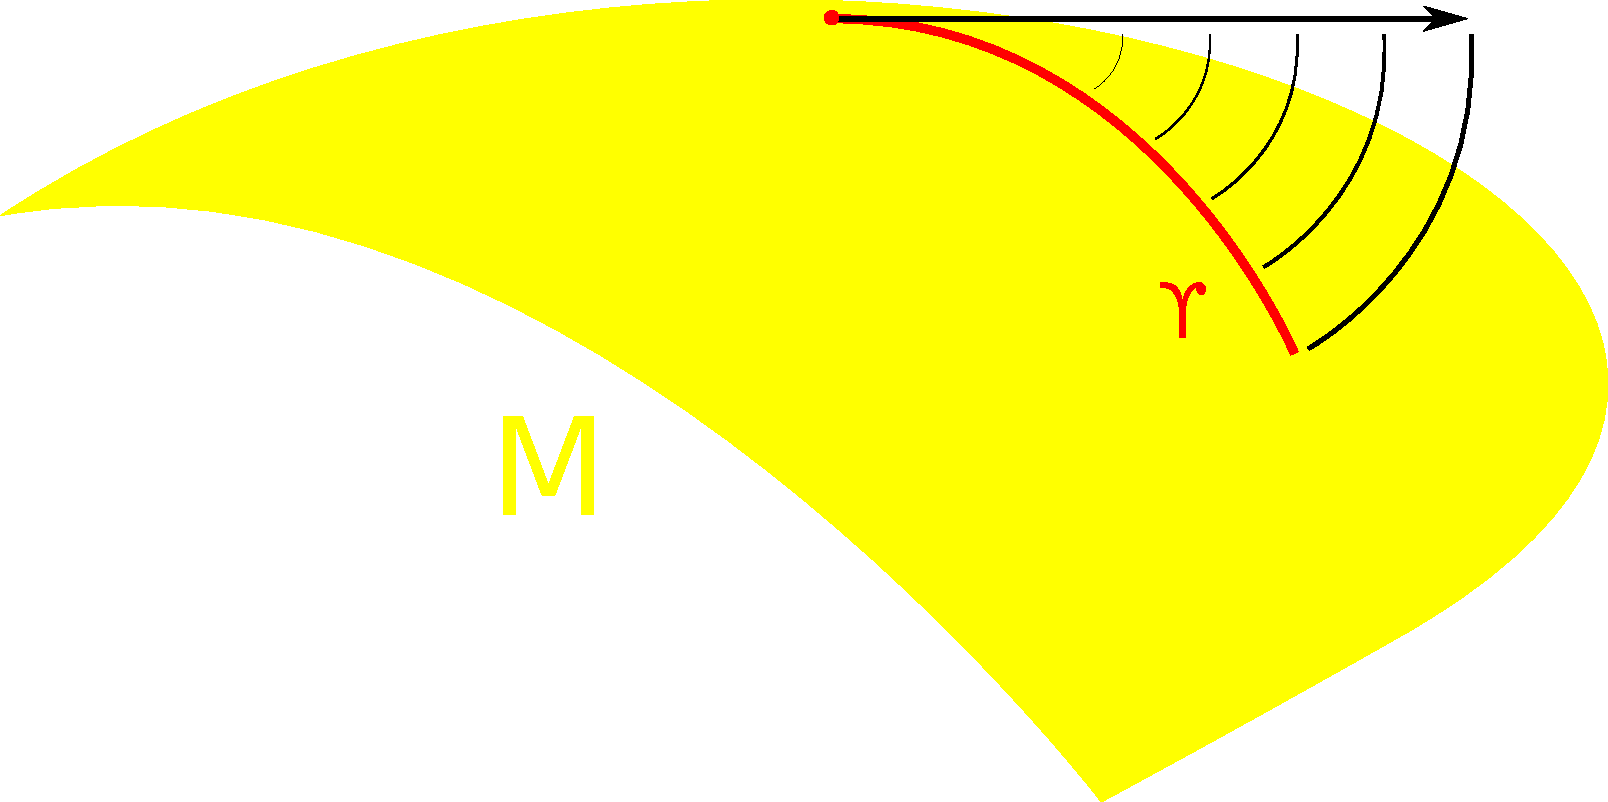
\includegraphics[scale=0.3]{fibrado_tang.pdf}
    \caption{Homotopy equivalence between a geodesic $\gamma\in M^{I}$ and its tangent vector at $\gamma(0)$.}
    \end{figure}

    Thus, Proposition \ref{fht_tang} allows us to state that the notion of tangent bundle can be extended from the concept of smooth 
    manifolds to topological manifolds.

    \begin{prop}\label{iso_homeo}
    If $h:M\to N$ is a homeomorphism between topological manifolds, then $(\tau M,\tau_{0}M)\sim_{f}h^{*}(\tau N,\tau_{0}N)$.
    \end{prop}

    \begin{proof}
        
    \

    Since $h$ is a homeomorphism, the map $H:(TM,T_{0}M)\to (TN,T_{0}N)$ given by $H(\omega)=h\circ\omega$ is one ass well, with inverse 
    $H^{-1}(\omega)=h^{-1}\circ\omega$.

    If we denote by $p:TM\to M$ and $q:TN\to N$ the projections of $(\tau M,\tau_{0}M)$ and $(\tau N,\tau_{0}N)$, respectively, then the 
    map $h^{-1}\circ q\circ H:TM\to M$ satisfies $h^{-1}\circ q\circ H(\omega)=p(\omega)$.

    Thus, Lemma \ref{iso_homot_2} guarantees that $(\tau M,\tau_{0}M)\sim_{f}h^{*}(\tau N,\tau_{0}N)$.

    \end{proof}

    Let us now see that the notion of generalized tangent bundle is natural with respect to the Cartesian product of topological manifolds, 
    in the following sense:

    \begin{prop}\label{fht_tang_cart}
        Let $M$ and $S$ be two arbitrary topological manifolds. Then:
        
        $$ (\tau (M\times S),\tau_{0}(M\times S))\sim_{f} (\tau M,\tau_{0}M)\times (\tau S,\tau_{0}S) $$
    \end{prop}
    \begin{proof}

    \

    Initially, consider $(\tau M,\tau_{0}M)=(TM,T_{0}M,p,M)$, $(\tau S,\tau_{0}S)=(TS,T_{0}S,q,S)$, and 
    $(\tau (M\times S),\tau_{0}(M\times S))=(T(M\times S),T_{0}(M\times S),r,M\times S)$. Denote the product 
    $(\tau M,\tau_{0}M)\times (\tau S,\tau_{0}S)=(E,E_{0},p\times q,M\times S)$, where:
    $$ E=(TM)\times(TS) $$
    $$ E_{0}=[(TM)\times (T_{0}S)]\bigcup [(T_{0}M)\times (TS)] $$

    \

    Consequently, the map $\phi:(T(M\times S),T_{0}(M\times S))\to (E,E_{0})$ defined by $\phi(\omega)=(p_{1}\circ\omega,p_{2}\circ\omega)$ 
    is well defined, because if $\omega\in T_{0}(M\times S)$, then $\omega(t)\neq \omega(0)$ for all $0<t\leq 1$. That is, $p_{i}\circ\omega(t)\neq p_{i}\circ\omega(0)$ for all $0<t\leq 1$ and $i=1$ or $2$, and thus, $p_{i}\circ\omega\in E_{0}$ for $i=1$ or $2$.

    On the other hand, observe that $\phi$ is a homeomorphism whose inverse map $\phi^{-1}:(E,E_{0})\to (T(M\times S),T_{0}(M\times S))$ is 
    naturally given by $\phi^{-1}(\omega_{1},\omega_{2})=(\omega_{1},\omega_{2})$. Moreover, it is clear that $(p\times q)\circ\phi=r$.

    Thus, it follows from Lemma \ref{iso_homot} that:
    $$(\tau (M\times S),\tau_{0}(M\times S))\sim_{f} (\tau M,\tau_{0}M)\times (\tau S,\tau_{0}S)$$

    \end{proof}



    \subsection{Generalized Normal Bundle of a Local-Flat Embedding}\label{secao_fht_normal}

    \

    In this subsection, we will show that the concept of generalized bundle\index{bundle!generalized} also allows the generalization of the 
    notion of normal vector bundle\index{bundle!vector!normal} from smooth manifolds\index{manifold!smooth} to topological 
    manifolds\index{manifold!topological}.

    Before moving forward, we recall\footnote{For more details, see (\cite{lee_s}, Proposition 5.16, p. 106).} that if \( M^{m} \) and 
    \( S^{m+k} \) are smooth manifolds and if \( i:M\hookrightarrow S \) is a smooth embedding\index{embedding!smooth}, then \( i(M) \) 
    constitutes a smooth submanifold of \( S \) such that, for every \( b\in M \), there exists an open neighborhood \( U\subset S \) of 
    \( i(b) \) with \( (U,U\cap i(M))\approx (\mathbb{R}^{m+k},\mathbb{R}^{m}) \).
    
    This feature leads us to the following:
    
    \begin{defi}
        A topological embedding\index{embedding!topological} \( i:M^{m}\hookrightarrow S^{m+k} \), between topological manifolds, is said to 
        be locally-flat, or simply local-flat\index{embedding!local-flat}, if for every \( b\in M \), there exists an open neighborhood 
        \( U\subset S \) of \( i(b) \) such that \( (U,U\cap i(M))\approx (\mathbb{R}^{m+k},\mathbb{R}^{m}) \).
    \end{defi}
    
    In the notation of the definition above, since \( M\approx i(M) \), we can rewrite \( M^{m}\subset S^{m+k} \) as a local-flat embedding 
    such that \( (U,U\cap M)\approx (\mathbb{R}^{m+k},\mathbb{R}^{m}) \). The notation used to describe a local-flat embedding will depend 
    on the problem at hand.

    \
    
    For the next result, consider:
    \begin{itemize}
        \item $M^{m}\subset S^{m+k}$ a local-flat embedding
        \item $N_{0}=\{ \omega\in S^{I} \ : \ \omega(t)\in M \Leftrightarrow t=0 \}$
        \item $N=N_{0}\bigcup \{ \omega\in S^{I} \ : \ \omega(t)=\omega(0)\in M, \ \forall t\in I \}$
        \item $q:N\to M$ given by $q(\omega)=\omega(0)$
    \end{itemize}

    \
    
    Thus:
    
    \begin{prop}
        Let $M^{m}\subset S^{m+k}$ be a local-flat embedding\index{embedding!local-flat}. Then, the pair 
        $(\mathcal{N},\mathcal{N}_{0})=(N,N_{0},q,M)$ is a locally trivial\index{locally trivial} $\R^{k}-$generalized bundle.
    \end{prop}
    
    The proof of the proposition above can be found in (\cite{fadell_1}, Proposition 4.1, p. 496).
    
    \begin{defi}
        We call $(\mathcal{N},\mathcal{N}_{0})$ the $\R^{k}-$generalized normal bundle\index{bundle!generalized!normal} of the local-flat 
        embedding $M^{m}\subset S^{m+k}$.
    \end{defi}
    
    On the other hand, consider $M^{m}\subset\R^{m+k}$ a smooth embedding\index{embedding!smooth} of a smooth manifold\index{manifold!smooth} 
    into Euclidean space, and let $\eta$ be the normal $\R^{k}$-vector bundle\index{bundle!vector!normal} of this embedding, as in 
    Definition \ref{defi_fvn}. Thus, we have the following relation between the normal vector bundle and the generalized normal bundle of the 
    local-flat embedding $M\subset \R^{m+k}$:
    
    \begin{prop}
        $(\eta,\eta_{0})\sim_{f} (\mathcal{N},\mathcal{N}_{0})$
    \end{prop}
    
    The proof of the proposition above can be found in (\cite{fadell_1}, Corollary 4.9, p. 498).
    
    In (\cite{fadell_1}, Theorem 4.11, p. 498), Fadell shows that Theorem \ref{dualidade_whitney_vet} is valid in the context of local-flat 
    embeddings, as follows:
    
    \begin{teo}\label{iso_merg_lf_1}
        If $M^{m}\subset S^{m+k}$ is a local-flat embedding with $\R^{k}-$generalized normal bundle $(\mathcal{N},\mathcal{N}_{0})$, then:
        $$ (\tau M,\tau_{0}M)\oplus (\mathcal{N},\mathcal{N}_{0})\sim_{f} (\tau S,\tau_{0}S)_{|M} $$
    \end{teo}
    
    Furthermore, we can obtain the following:

    \begin{prop}\label{iso_merg_lf_2}
        If $i:M^{m}\hookrightarrow S^{m+k}$ is a local-flat embedding\index{embedding!local-flat}, then:
        $$ (\tau S,\tau_{0}S)_{|M}\sim_{f} i^{*}(\tau S,\tau_{0}S) $$
    \end{prop}
    \begin{proof}

        \
        
        First, let us fix the following notations:
        
        \begin{enumerate}
            \item $(\tau S,\tau_{0}S)=(T,T_{0},p,S)$, where:
            \begin{itemize}
                \item $T_{0}=\{ \omega\in S^{I} \ : \ \omega(t)=\omega(0) \Leftrightarrow t=0 \}$
                \item $T=T_{0}\bigcup \{ \omega\in S^{I} \ : \ \omega(t)=\omega(0), \ \forall t\in I \}$
                \item $p:T\to S$ given by $p(\omega)=\omega(0)$
            \end{itemize}
            \item $(\tau S,\tau_{0}S)_{|M}=(p^{-1}(M),p^{-1}(M)\cap T_{0},q,M)$, where:
            \begin{itemize}
                \item $p^{-1}(M)=\{ \omega\in T \ : \ \omega(0)\in M \}$
                \item $p^{-1}(M)\cap T_{0}=\{ \omega\in T_{0} \ : \ \omega(0)\in M \}$
                \item $q=p_{|p^{-1}(M)}:p^{-1}(M)\to M$ given by $q(\omega)=\omega(0)$
            \end{itemize}
            \item $i^{*}(\tau S,\tau_{0}S)=(i^{*}T,i^{*}T_{0},p_{1},M)$, where:
            \begin{itemize}
                \item $i^{*}T=\{ (b,\omega)\in M\times T \ : \ i(b)=\omega(0) \}$
                \item $i^{*}T_{0}=\{ (b,\omega)\in i^{*}T \ : \ \omega\in T_{0} \}$
                \item $p_{1}:i^{*}T\to M$ given by $p_{1}(b,\omega)=b$
            \end{itemize}
        \end{enumerate}
        
        Thus, the fiber map $\phi:(p^{-1}(M),p^{-1}(M)\cap T_{0})\to (i^{*}T,i^{*}T_{0})$ given by $\phi(\omega)=(\omega(0),\omega)$ is 
        well-defined.

        On the other hand, note that the map $\psi:(i^{*}T,i^{*}T_{0})\to (p^{-1}(M),p^{-1}(M)\cap T_{0})$ given by $\psi(b,\omega)=\omega$ is 
        also well-defined.
        
        Furthermore, it is clear that $\phi$ is a homeomorphism with inverse $\psi$. Thus, Lemma \ref{iso_homot} guarantees that 
        $(\tau S,\tau_{0}S)_{|M}\sim_{f} i^{*}(\tau S,\tau_{0}S)$.
        
    \end{proof}

    \
    
    With this, we conclude in this chapter the study of generalized bundles\index{bundle!generalized}, a concept developed by Fadell in \cite{fadell_1} to generalize the notions of tangent\index{bundle!vector!tangent} and normal\index{bundle!vector!normal} vector bundles from the context of smooth manifolds\index{manifold!smooth} to topological manifolds\index{manifold!topological}, where we presented here only the intuitive proof, based on Nash's ideas in \cite{nash}, of how the generalization of the tangent vector bundle occurs.
    
    In order to not only present a modern reinterpretation of the first half of the results presented by Fadell in \cite{fadell_1}, but also to complement \cite{fadell_1}, we have carefully shown in detail how the generalized bundles indeed generalize vector bundles\index{bundle!vector}, as well as how the notion of vector bundle isomorphism is preserved when extended to the category of generalized bundles.
    
    It is worth noting that we also developed in this chapter the concept of pullback generalized bundle\index{bundle!generalized!pullback}, as well as some consequences of such a bundle, a concept that was not mentioned by Fadell in \cite{fadell_1}.
    
    In any case, the results about generalized bundles carefully developed in this chapter suggest that we view this concept as a theory in itself and not just as a tool to construct characteristic classes, as we will present in the following chapter.
    


    \chapter{Characteristic Classes of Topological Manifolds}\label{cap_clas_carac}
    \thispagestyle{empty}
    
    \
    
    In this chapter, we will construct the Thom\index{class!Thom} classes, Stiefel-Whitney\index{class!Stiefel-Whitney} classes, and 
    Euler\index{class!Euler} classes of generalized bundles\index{bundle!generalized}, and present some consequences of such objects. 
    In particular, we will examine the behavior of these classes for the generalized tangent bundles\index{bundle!generalized!tangent} of 
    topological manifolds\index{manifold!topological}.
    
    To that end, in Section \ref{secao_thom}, we will introduce the concept of orientability of generalized bundles, which was originally 
    proposed by Fadell in \cite{fadell_1}, in order to guarantee the existence of the Thom class and Thom isomorphism for such bundles. 
    We will also discuss how the Thom class behaves in specific generalized bundles.
    
    In Section \ref{secao_SW}, we will define the Stiefel-Whitney classes of generalized bundles in a manner identical to the definition of 
    the Stiefel-Whitney classes of vector bundles\index{bundle!vector} presented in \cite{milnor_1}. Furthermore, we will see how the notion 
    of pullback generalized bundle introduced in the previous chapter will be relevant to deduce some consequences concerning the 
    Stiefel-Whitney classes, since Fadell did not address this concept in \cite{fadell_1}.
    
    Concluding the chapter, in Section \ref{secao_euler}, we will define the Euler class of generalized bundles, a topic that was scarcely 
    addressed by Fadell in \cite{fadell_1}. In this section, we will present several well-known results about Euler classes of vector 
    bundles and smooth manifolds, but in their versions for generalized bundles and topological manifolds.
    
    As explained in Remark \ref{obs_varied_bordo}, we emphasize that every topological manifold mentioned in this chapter will be a 
    manifold without boundary.
    


    \section{Orientability and Thom Class}\label{secao_thom}

    \

    A







    \chapter{Applications in Closed Topological Manifolds}\label{cap_aplic}
    \thispagestyle{empty}



    \chapter{Characteristic Classes of Generalized Manifolds}\label{cap_wu_gen}
    \thispagestyle{empty}



    \appendix

    \chapter{Singular (Co)homology}\label{ap_(co)_sing}
    \thispagestyle{empty}

    \

    In order to keep this work concise, yet complete and self-explanatory, we will use this appendix as 
    a brief review of some well-known concepts from Algebraic Topology.

    When referring simultaneously to the singular homology and cohomology modules, for convenience, we 
    will simply write singular (co)homology modules\index{singular (co)homology}. Thus, we ask the 
    reader to already be familiar with the concepts of these theories.
    
    \section{Main results}\label{ap_principais_res}
    
    We will use this section to state general results on singular (co)homology that will be useful for 
    the development of this work and for a better understanding of the constructions made in the 
    following sections of this appendix.
    
    \begin{teo}{\bf (Universal Coefficients)\index{theorem!of Universal Coefficients}}
        Let $(X,A)$ be any pair of topological spaces. Then:
        \begin{enumerate}
            \item \textbf{(general case for homology)\footnote{Can be found in (\cite{hatcher}, 
            Corollary 3A.4, p. 264).}} If $H_{k}(X,A;\Z)$ is a free 
            module\footnote{A module is called free if it admits a basis.}\index{module!free} for 
            all $k\geq 0$ or $R$ is a free module, then:
            $$ H_{k}(X,A;R)\cong H_{k}(X,A;\Z)\tensor R, \ \forall k\geq 0 $$
            \item \textbf{(general case for cohomology)\footnote{Can be found in (\cite{hatcher}, 
            Theorem 3.2, p. 195).}} If $H_{k}(X,A;\Z)$ is a free module for all $k\geq 0$, then:
            $$ H^{k}(X,A;R)\cong Hom(H_{k}(X,A;\Z);R), \ \forall k\geq 0 $$
            \item \textbf{(particular case)\footnote{Can be found in (\cite{hatcher}, p. 198).}} 
            If $\mathbb{F}$ is a field, then the Kronecker product ensures that:
            $$ H^{k}(X,A;\F)\cong Hom(H_{k}(X,A;\F);\F), \ \forall k\geq 0 $$
        \end{enumerate}
        For $R=\Z$ in case 2 or $R=\F$ in case 3, the isomorphism is given by the relation 
        $x\in H^{k}(X,A;R)\mapsto\overline{x}(a)=<x,a>\in R$.
    \end{teo}
    
    \begin{teo}{\bf (Künneth Formula)\index{formula!of Künneth}}
        Let $X$ and $Y$ be any topological spaces and $R$ a finitely generated principal ideal 
        domain\index{principal ideal domain}. Then:
        \begin{enumerate}
            \item \textbf{(case for absolute cohomology)\footnote{Can be found in (\cite{spanier}, 
            Theorem 1, p. 249).}} If all the singular homology $R$-modules of $Y$ are finitely 
            generated\index{module!finitely generated}, then:
            $$ H^{k}(X\times Y;R)\cong \ds\bigoplus_{i+j=k}\left[ H^{i}(X;R)\tensor H^{j}(Y;R)\right], \ 
            \forall k\geq 0 $$
            \item \textbf{(case for absolute homology)\footnote{Can be found in (\cite{spanier}, 
            Theorem 10, p. 235).}}
            $$ H_{k}(X\times Y;R)\cong \ds\bigoplus_{i+j=k}\left[ H_{i}(X;R)\tensor H_{j}(Y;R)\right], \ 
            \forall k\geq 0 $$
        \end{enumerate}
    \end{teo}
    
    The proofs of the general cases of the Universal Coefficients Theorem can be found in (\cite{spanier}, 
    Chapter 5, Sections 2 and 5).
    
    The proofs of the Künneth formulas, in their general versions for pairs, can be found in 
    (\cite{spanier}, Chapter 5, Sections 3 and 5).
    
    Now, let us briefly review some properties about the cap\index{product!cap}, cup\index{product!cup}, 
    cross\index{product!cross}, and Kronecker\index{product!Kronecker} products.

    \begin{lem}\label{propriedades_produtos}
        Let $X$, $X'$, $Y$, and $Y'$ be arbitrary topological spaces, $f:X\to X'$ and $g:Y\to Y'$ any 
        maps, $p_{1}:X\times Y\to X$ and $p_{2}:X\times Y\to Y$ the canonical projections, and 
        $d:X\to X\times X$ the diagonal map\index{map!diagonal}. If $a\in H_{q}(X;R)$, $b\in H_{r}(Y;R)$, 
        $x\in H^{i}(X;R)$, $x_{1}\in H^{i_{1}}(X;R)$, $x_{2}\in H^{i_{2}}(X;R)$, $y\in H^{j}(Y;R)$, 
        $y_{1}\in H^{j_{1}}(Y;R)$, $y_{2}\in H^{j_{2}}(Y;R)$, $a'\in H_{q'}(X;R)$, $x'\in H^{i'}(X';R)$, 
        $x'_{1}\in H^{i_{1}'}(X';R)$, $x'_{2}\in H^{i_{2}'}(X';R)$, $y'\in H^{j'}(Y';R)$, then:
    
        \begin{enumerate}
            \item $1\ccup x=x=x\ccup 1$
            \item $0\ccup x=0=x\ccup 0$
            \item $x_{1}\ccup x_{2}=0$ \  $\Longleftrightarrow$ \ $x_{1}=0$ or $x_{2}=0$, when $R=\Z_{2}$
            \item $a\ccap 1=a$
            \item $x_{1}\ccup x_{2}=(-1)^{|x_{1}|.|x_{2}|}(x_{2}\ccup x_{1})$
            \item $(a\ccap x_{1})\ccap x_{2}=a\ccap (x_{2}\ccup x_{1})$
            \item $(x_{1}\times y_{1})\ccup (x_{2}\times y_{2})=(-1)^{|y_{1}|.|x_{2}|}(x_{1}\ccup x_{2})\times (y_{1}\ccup y_{2})$
            \item $(a\times b)\ccap (x\times y)=(-1)^{|a|.(|y|-|b|)}(a\ccap x)\times (b\ccap y)$
            \item $<x_{1}\ccup x_{2},a>=<x_{1},a\ccap x_{2}>$
            \item $<x\times y,a\times b>=(-1)^{|x|.|y|}<x,a>.<y,b>$
            \item $p_{1}^{*}(x)=x\times 1$ and $p_{2}^{*}(y)=1\times y$
            \item $x\times y=p_{1}^{*}(x)\ccup p_{2}^{*}(y)$
            \item $x_{1}\ccup x_{2}=d^{*}(x_{1}\times x_{2})$
            \item $f_{*}(a\ccap f^{*}(x'))=f_{*}(a)\ccap x'$
            \item $(f\times g)^{*}(x'\times y')=f^{*}(x')\times g^{*}(y')$
            \item $f^{*}(x'_{1}\ccup x'_{2})=f^{*}(x'_{1})\ccup f^{*}(x'_{2})$
            \item $<f^{*}(x'),a>=<x',f_{*}(a)>$
            \item $<(f^{*})^{-1}(x),a'>=<x,(f_{*})^{-1}(a')>$, if $f^{*}$ and $f_{*}$ are isomorphisms.
        \end{enumerate}
    \end{lem}
    
    The properties in the lemma above can be found, in their general versions for pairs, in 
    (\cite{spanier}, Chapter 5).
    
    Moreover, item 16 of Lemma \ref{propriedades_produtos} admits a particular case when involving the 
    inclusion map, in the following sense:
    
    \begin{lem}\label{propriedades_produtos_2}
        Let $(X,A)$ and $j:X\hookrightarrow (X,A)$ be an arbitrary pair of topological spaces and the 
        canonical inclusion, respectively. Then, for any $x_{1}\in H^{i_{1}}(X;R)$ and $x_{2}\in H^{i_{2}}(X,A;R)$, 
        we have:
        $$ j^{*}(x_{1}\ccup x_{2})=x_{1}\ccup j^{*}(x_{2}) $$
    \end{lem}
    
    The proof of the lemma above can also be found in (\cite{spanier}, Chapter 5).
    
    That said, item 14 of Lemma \ref{propriedades_produtos} admits the following particular case:

    \begin{lem}\label{propriedades_produtos_3}
        Let $(X,A)$ be any pair of topological spaces and let $j:X\hookrightarrow (X,A)$ be the canonical inclusion. Then, for any 
        $x\in H^{i_{1}}(X,A;R)$ and $a\in H_{i_{2}}(X;R)$, we have:
        $$
        j_{*}(a)\ccap x = a\ccap j^{*}(x)
        $$
    \end{lem}
    
    \begin{proof}

        \

        It suffices to observe that, for any $y\in H^{i_{2}-i_{1}}(X;R)$, we have:

        \
        
        $\begin{array}{rl}
            \langle y, j_{*}(a)\ccap x \rangle & = \langle y\ccup x, j^{*}(a) \rangle \\
            & = \langle j^{*}(y\ccup x), a \rangle \\
            & = \langle y\ccup j^{*}(x), a \rangle \\
            & = \langle y, a\ccap j^{*}(x) \rangle
        \end{array}$

        \

        \
    
        Thus, the Universal Coefficient Theorem ensures that $j_{*}(a)\ccap x = a\ccap j^{*}(x)$.
    \end{proof}
    
    Now, also due to the Universal Coefficient Theorem\index{theorem!Universal Coefficient}, the 
    following result is a direct consequence of (\cite{hungerford}, Theorem 4.11, p. 204):
    
    \begin{prop}\label{prop_alg_comut}
        Let $R=\mathbb{Z}$ or $R=\mathbb{F}$ be any field, and let $(X,A)$ be any pair of topological 
        spaces such that $H_{k}(X,A;R)$ is a finitely generated 
        $R$-module\index{module!finitely generated} for all $k\geq 0$. Then, for any $k\geq 0$, 
        $\alpha\in R$ and $a\in H_{k}(X,A;R)$ with $a\neq 0$, there exists a unique $x\in H^{k}(X,A;R)$ 
        such that $x\neq 0$ and $\langle x, a \rangle = \alpha$.
    \end{prop}
    
    Proceeding, we will construct the cohomology ring of a pair $(X,A)$.
    
    \begin{defi}{\bf (Cohomology Ring)}
        We call $(H^{*}(X,A;R), +, \ccup)$ the cohomology ring\index{cohomology ring} of the pair 
        $(X,A)$ with coefficients in $R$, the set formed by the following formal infinite series:
        $$
        H^{*}(X,A;R) = \{ x = x_{0} + x_{1} + x_{2} + \ldots \ : \ x_{k}\in H^{k}(X,A;R), \ \forall 
        k\geq 0 \}
        $$
        
        Furthermore, given $x = x_{0} + x_{1} + x_{2} + \ldots$ and $y = y_{0} + y_{1} + y_{2} + \ldots$ 
        in $H^{*}(X,A;R)$, the operations that define this ring are given by:
        
        \begin{enumerate}
            \item $x + y = z_{0} + z_{1} + z_{2} + \ldots$, where $z_{k} = x_{k} + y_{k}$ for all 
            $k\geq 0$
            \item $x\ccup y = z_{0} + z_{1} + z_{2} + \ldots$, where $z_{k} = 
            \displaystyle\sum_{i+j=k} x_{i}\ccup y_{j}$ for all $k\geq 0$
        \end{enumerate}
    \end{defi}

    Since the cup product is a commutative operation when $R=\Z_{2}$, then $H^{*}(X,A;\Z_{2})$ will be a commutative ring with identity 
    element $1+0+0+\dots\in H^{*}(X,A;\Z_{2})$.

    \begin{teo}\label{teo_elemento_inversivel}
        The units of the ring $H^{*}(X,A;\Z_{2})$ are elements of the following form:
        $$ x=x_{0}+x_{1}+x_{2}+\dots\in H^{*}(X,A;\Z_{2}) \ : \ x_{0}=1 $$
        
        Furthermore, the inverse of a unit $x=1+x_{1}+x_{2}+\dots$ is the following element:
        $$ x^{-1}=1+x^{-1}_{1}+x^{-1}_{2}+\dots, \quad \text{where} \quad x^{-1}_{k}=\ds\sum_{\stackrel{i+j=k}{i\neq 0}}x_{i}\ccup 
        x^{-1}_{j}, \ \forall k\geq 1 $$
    \end{teo}
    
    The proof of the theorem above can be found in (\cite{alex}, Lemma 6.1, p. 53).
    
    At this point, let us see when a topological space has all its singular (co)homology modules finitely generated and under which conditions 
    we can define the Euler characteristic of an arbitrary topological space.
    
    \begin{prop}
        All singular homology modules of a compact ENR space\footnote{An ENR is a topological space that is a retract\index{retract} of an open 
        neighborhood in some Euclidean space, that is, it can be embedded in some Euclidean space as a retract of an open neighborhood of that 
        Euclidean space. More details about these spaces can be found in (\cite{dold}, Chapter 4, Section 8).}\index{ENR} are finitely 
        generated\index{module!finitely generated}.
    \end{prop}
    
    The proof of the proposition above can be found in (\cite{hatcher}, Corollary A.8, p. 527). As a particular consequence, all singular 
    homology modules of a compact topological manifold are free, since every topological manifold\index{manifold!topological} is an ENR and 
    every finitely generated module is free\index{module!free}. Furthermore, due to the Universal Coefficient Theorem, every singular 
    cohomology module of a compact topological manifold is free.
    
    \begin{defi}{\bf (Euler Characteristic)}
        Let $X$ be a topological space such that there exists an integer $n>0$ such that $H_{k}(X;\Z)=0$ for $k>n$ and $H_{k}(X;\Z)$ is a 
        finitely generated $\Z$-module for every $0\leq k\leq n$. Thus, the Euler characteristic\index{Euler characteristic} of $X$ is given 
        by the following alternating sum:
        $$ \chi(X)=\ds\sum_{k=0}^{n}(-1)^{k}\operatorname{rank}(H_{k}(X;\Z)) $$
    \end{defi}
    
    Due to the Universal Coefficient Theorem\index{theorem!Universal Coefficient Theorem}, the Euler characteristic of a space $X$ under the 
    conditions of the definition above can be computed using singular homology modules with coefficients in any field $\F$ as follows:
    $$ \chi(X)=\ds\sum_{k=0}^{n}(-1)^{k}\dim(H_{k}(X;\F)) $$
    
    To conclude this section, let us make some considerations about the infinite real projective space\index{real projective space!infinite} 
    $\RP^{\infty}$, which will be useful for calculating the Stiefel–Whitney classes\index{class!Stiefel–Whitney} of real projective spaces 
    using the topological version of Wu's formula\index{formula!Wu}.
    
    Denoting by $\RP^{k}$ the $k$-dimensional real projective space\index{real projective space!finite}, we can define the infinite real 
    projective space $\RP^{\infty}$ as the direct limit of the following sequence:
    $$ \RP^{0} \subset \RP^{1} \subset \cdots \subset \RP^{k} \subset \cdots $$
    
    In other words, we have that $\RP^{\infty}=\ds\bigcup_{k\geq 0}\RP^{k}$, endowed with the following topology:
    
    \begin{center}
        "$U$ is an open subset of $\RP^{\infty}$ if and only if $U\cap\RP^{k}$ is an open subset of $\RP^{k}$ for every $k\geq 0$."
    \end{center}
    
    Thus, we can state the following:
    
    \begin{lem}\label{iso_proj}
        The canonical inclusion $i:\RP^{n}\hookrightarrow \RP^{\infty}$ gives rise to an isomorphism 
        $i^{*}:H^{k}(\RP^{\infty};\Z_{2})\to H^{k}(\RP^{n};\Z_{2})$ for every $0\leq k\leq n$.
    \end{lem}
    
    \begin{proof}
    
    First, recall that $\RP^{n+1}$ is a CW-complex\index{CW-complex} with one open cell in each dimension, with $\RP^{k}$ being its 
    $k$-skeleton.
    
    Now, consider $e_{n+1}$ as the open $(n+1)$-dimensional cell of $\RP^{n+1}$ and fix $x\in e_{n+1}$. Then, $\RP^{n+1}-\{ x \}$ is a 
    deformation retract\index{deformation retract} of $\RP^{n}$.
    
    On the other hand, considering, up to homeomorphism, $x\in D^{n+1}\subset e_{n+1}$, then $U=\RP^{n+1}-D^{n+1}$ will be an open subspace 
    of $\RP^{n+1}$ such that:
    $$ \overline{U}\subset \operatorname{int}(\RP^{n+1}-\{ x \})=\RP^{n+1}-\{ x \}. $$
    
    Thus, $\mathbb{S}^{n}=\partial D^{n+1}$ is a deformation retract of $(\RP^{n+1}-\{ x \})-U=D^{n+1}-\{ x \}$, and we also obtain the 
    following excision:
    $$ (\RP^{n+1}-U,(\RP^{n+1}-\{ x \})-U)\hookrightarrow (\RP^{n+1},\RP^{n+1}-\{ x \}). $$
    
    Therefore, we have the following isomorphisms:
    
    \[
    \begin{array}{rl}
    H^{k}(\RP^{n+1},\RP^{n};\Z_{2}) \ \cong & H^{k}(\RP^{n+1},\RP^{n+1}-\{ x \};\Z_{2}) \\[8pt]
    \cong & H^{k}(\RP^{n+1}-U,(\RP^{n+1}-\{ x \})-U;\Z_{2}) \\[8pt]
    \cong & H^{k}(D^{n+1},\mathbb{S}^{n};\Z_{2}) \\[8pt]
    \cong & \left\{
    \begin{array}{cl}
    \Z_{2} & ,\quad k=n+1 \\
    0      & ,\quad k\neq n+1
    \end{array}
    \right.
    \end{array}
    \]
    
    In particular, $H^{k}(\RP^{n+1},\RP^{n};\Z_{2})=0$ for $0\leq k\leq n$. From now on in this proof, fix $0\leq k\leq n$.
    
    Now, we prove by induction on $t\geq 2$ that $H^{k}(\RP^{n+t},\RP^{n};\Z_{2})=0$.
    
    To do so, consider initially the long exact cohomology sequence of the triple\footnote{For more details about the long exact cohomology 
    sequence of a triple, see (\cite{hatcher}, p. 200).} $(\RP^{n+2},\RP^{n+1},\RP^{n})$:
    $$ \cdots \to H^{k}(\RP^{n+2},\RP^{n+1};\Z_{2}) \to H^{k}(\RP^{n+2},\RP^{n};\Z_{2}) \to H^{k}(\RP^{n+1},\RP^{n};\Z_{2}) \to \cdots $$
    
    Since $H^{k}(\RP^{n+2},\RP^{n+1};\Z_{2})=0=H^{k}(\RP^{n+1},\RP^{n};\Z_{2})$, the exactness of the sequence above ensures that 
    $H^{k}(\RP^{n+2},\RP^{n};\Z_{2})=0$.
    
    Thus, assuming $H^{k}(\RP^{n+t_{0}},\RP^{n};\Z_{2})=0$ for some $t_{0}>2$, we similarly obtain that 
    $H^{k}(\RP^{n+(t_{0}+1)},\RP^{n};\Z_{2})=0$, simply by using the long exact cohomology sequence of the triple 
    $(\RP^{n+(t_{0}+1)},\RP^{n+t_{0}},\RP^{n})$.
    
    Therefore, we conclude that $H^{k}(\RP^{n+t},\RP^{n};\Z_{2})=0$ for any $t\geq 0$. Consequently:
    $$ H^{k}(\RP^{\infty},\RP^{n};\Z_{2})=\lim_{\longrightarrow}H^{k}(\RP^{n+t},\RP^{n};\Z_{2})=0. $$
    
    Finally, consider the long exact cohomology sequence of the pair $(\RP^{\infty},\RP^{n})$:
    $$
    \xymatrix @C=0.5cm {
    \cdots \ar[rr] && H^{k}(\RP^{\infty},\RP^{n};\Z_{2}) \ar[rr] && H^{k}(\RP^{\infty};\Z_{2}) \ar[rr]^-{i^{*}} && H^{k}(\RP^{n};\Z_{2}) \ar[rr] && \cdots
    }
    $$
    
    Since $H^{k}(\RP^{\infty},\RP^{n};\Z_{2})=0$ and $H^{k}(\RP^{\infty};\Z_{2})\cong\Z_{2}\cong H^{k}(\RP^{n};\Z_{2})$, then $i^{*}$ is a 
    monomorphism between modules of the same dimension, that is, $i^{*}$ is an isomorphism.
    
    \end{proof}



    \section{Slant Product}\label{ap_slant}

    In this section, we will define a specific product between singular (co)homology modules that will be fundamental in the proof of the Wu 
    formula\index{formula!Wu's formula} for topological\index{manifold!topological} and homological\index{manifold!homological} manifolds.

    This product, which we will later call the slant product, is defined for arbitrary topological spaces using singular (co)homology modules 
    with coefficients in an arbitrary commutative unital ring, and it is also used in the proof of the Wu formula for smooth 
    manifolds\index{manifold!smooth}, as seen in (\cite{milnor_1}, Chapter 11).
    
    For our context, let $R=\Z$ or $R=\Z_{2}$, $X$ and $Y$ be arbitrary topological spaces with $H_{k}(Y;R)$ finitely generated for all 
    $k\geq 0$, and integers $i,j\geq 0$. Thus, define the following homomorphism involving $R$-modules of singular (co)homology:
    $$ H^{i}(X;R)\tensor H^{j}(Y;R)\tensor H_{j}(Y;R)\to H^{i}(X;R) $$
    $$ x\tensor y\tensor b\mapsto <y,b>x $$
    
    Now, the Künneth formula\index{formula!Künneth formula} ensures that $H^{*}(X\times Y;R)\cong H^{*}(X;R)\tensor H^{*}(Y;R)$, and since 
    $H^{*}(X\times Y;R)$ is a ring generated by elements of the form $x\times y$, the following homomorphism is well defined:

    \newpage
    $$ H^{i+j}(X\times Y;R)\tensor H_{j}(Y;R)\to H^{i}(X;R) $$
    $$ (x\times y)\tensor b\mapsto (x\times y)/b=<y,b>x $$
    
    Thus, we have the following:
    
    \begin{defi}{\bf (Slant Product)}
        The slant product\index{product!slant} refers to the homomorphism $H^{i+j}(X\times Y;R)\tensor H_{j}(Y;R)\to H^{i}(X;R)$ given by 
        $z\tensor b\mapsto z/b$.
    \end{defi}
    
    We will conclude this section with two particular properties of the slant product. For more details about this operation in its most 
    general form, we suggest the reader see (\cite{spanier}, Chapter 6, Section 1).
    
    \begin{lem}\label{lema_slant}
        Let $x\times 1\in H^{i}(X\times Y;R)$, $z\in H^{i+j}(X\times Y;R)$, $a\in H_{i'}(X;R)$, $b\in H_{j}(Y;R)$, and $p_{1}:X\times Y\to X$ 
        be the canonical projection. Then, we have the following relations:
        
        \begin{enumerate}
            \item $[(x\times 1)\ccup z]/b=x\ccup(z /b)$
            \item $(p_{1})_{*}((a\times b)\ccap z)=a\ccap (z/b)$
        \end{enumerate}
    \end{lem}

    

    \section{Steenrod Squares}\label{ap_steenrod}

    \

    The Steenrod squares\index{Steenrod square} are cohomological operations of great importance for the development of this work, as they 
    are essential for defining the Stiefel-Whitney classes\index{Stiefel-Whitney class} of vector bundles\index{vector bundle}, 
    generalized\index{generalized bundle}, and homological\index{homological variety} manifolds\index{manifold}. Furthermore, the Wu 
    formula\index{Wu formula} relates, through these Steenrod squares, the Stiefel-Whitney and Wu classes of a smooth\index{smooth manifold}, 
    topological\index{topological manifold}, and homological variety.

    Here, we will state only the basic properties of these operations. For more details on Steenrod squares, we refer the reader to 
    (\cite{spanier}, Chapter 5, Section 9).
    
    Given $(X,A)$ a pair of topological spaces and integers $m,k\geq 0$, the Steenrod squares are additive cohomological operations 
    $Sq^{k}:H^{m}(X,A;\Z_{2})\to H^{m+k}(X,A;\Z_{2})$ satisfying the following properties:
    
    \begin{enumerate}
        \item If $x\in H^{m}(X,A;\Z_{2})$ and $y\in H^{n}(X,A;\Z_{2})$, then the Cartan formula\index{Cartan formula} holds, i.e., 
        $$ Sq^{k}(x\ccup y)=\ds\sum_{i+j=k}Sq^{i}(x)\ccup Sq^{j}(y) $$	
        \item If $x\in H^{m}(X,A;\Z_{2})$, then: 
        \begin{enumerate}
            \item $Sq^{0}(x)=x$		
            \item $Sq^{m}(x)=x\ccup x$		
            \item $Sq^{k}(x)=0$, for $k>m$
        \end{enumerate}
        
        \item If $f:(X,A)\to (Y,B)$ is a map of pairs, then $Sq^{k}\circ f^{*}=f^{*}\circ Sq^{k}$, i.e., the following diagram commutes:
        $$\xymatrix @C=0.5cm {
            H^{m}(Y,B;\Z_{2}) \ar[rrr]^{f^{*}} \ar[dd]_{Sq^{k}} & & & H^{m}(X,A;\Z_{2}) \ar[dd]_{Sq^{k}} \\
            & & & \\
            H^{m+k}(Y,B;\Z_{2}) \ar[rrr]^{f^{*}} & & & H^{m+k}(X,A;\Z_{2})
        }$$ 
    \end{enumerate}
    
    Furthermore, if $f:(X,A)\to (Y,B)$ is a map that induces an isomorphism in the context of $\Z_{2}$-modules of singular cohomology, then 
    it follows from the property above that:
    $$ Sq^{k}\circ(f^{*})^{-1}=(f^{*})^{-1}\circ Sq^{k} $$
    
    On the other hand, given $x\in H^{m}(X,A;\Z_{2})$, we can define the total square operation as follows:
    $$ Sq(x)=x+Sq^{1}(x)+Sq^{2}(x)+...+Sq^{m}(x) $$
    
    Thus, for any $x\in H^{m}(X,A;\Z_{2})$ and $y\in H^{n}(X,A;\Z_{2})$, the Cartan formula\index{Cartan formula} can be rewritten as:
    $$ Sq(x\ccup y)=Sq(x)\ccup Sq(y) $$
    
    To conclude this section, given $x\in H^{m}(X,A;\Z_{2})$ and $y\in H^{n}(Y,B;\Z_{2})$, we can derive, using the cross 
    product\index{cross product} and the Cartan formula, the following relations:
    $$ Sq^{k}(x\times y)=\ds\sum_{i+j=k}Sq^{i}(x)\times Sq^{k}(y) $$ 
    $$ Sq(x\times y)=Sq(x)\times Sq(y) $$
    
    

    \section{$R-$Orientation Classes and e Dualities}\label{ap_orient}

    \

    In this section, we will define the notion of $R$-orientability of a topological manifold\index{manifold!topological} and state some 
    results in this context. Afterward, we will present the most important results involving topological manifolds in the realm of 
    (co)homology\index{(co)homology} theory, known as dualities.

    For a more detailed reading on orientations and the dualities mentioned here, we suggest (\cite{hatcher}, Chapter 3, Section 3.3).
    
    \begin{defi}{\bf (Local Orientation)}
        Consider $M^{m}$ a topological manifold. Then:
        \begin{enumerate}
            \item An $R$-local orientation\index{orientation!local} of $M$ at $b \in M$ is the choice of a generator which we denote by 
            $([M]_{b}) = H_{m}(M, M-\{b\}; R) \cong R$.
            \item An $R$-local orientation of $M$ along a subspace $U \subset M$ is the choice of an element $[M]_{U} \in H_{m}(M, M-U; R)$ 
            such that, for all $b \in U$, we have $((j_{b}^{U})_{*}([M]_{U})) = H_{m}(M, M-\{b\}; R)$, where 
            $j_{b}^{U}:(M, M-U) \hookrightarrow (M, M-\{b\})$ is the canonical inclusion.
        \end{enumerate}
        
        The elements $[M]_{b}$ and $[M]_{U}$ are called the classes of local $R$-orientation\index{class!of local orientation} of $M$ at 
        $b \in M$ and along $U$, respectively.
    \end{defi}
    
    \begin{defi}{\bf (Global Orientation\index{orientation!global})}
        A topological manifold $M^{m}$ is said to be $R$-orientable if there exists an open cover $\mathcal{U}$ of $M$ such that:
        \begin{enumerate}
            \item if $U_{i}, U_{j} \in \mathcal{U}$ and $b \in U_{i} \cap U_{j}$, then 
            $(j_{b}^{U_{i}})_{*}([M]_{U_{i}}) = (j_{b}^{U_{j}})_{*}([M]_{U_{j}})$.
            \item for every $U \in \mathcal{U}$ and $b \in U$, we have $[M]_{b} = (j_{b}^{U})_{*}([M]_{U})$
        \end{enumerate}
    \end{defi}
    
    After defining local and global orientations, let us consider the following:
    
    \begin{prop}\label{orient_local}
        Let $M^{m}$ be an $R$-orientable topological manifold. Then:
        \begin{enumerate}
            \item If $M$ is connected and closed, the inclusion $j_{b}^{M} = j_{b}: M \hookrightarrow (M, M-\{b\})$ is such that 
            $(j_{b})_{*}: H_{m}(M; R) \to H_{m}(M, M-\{b\}; R)$ is an isomorphism for all $b \in M$.
            \item For each compact $K \subset M$, there exists a unique class of $R$-local orientation of $M$ along 
            $K$, $[M]_{K} \in H_{m}(M, M-K; R)$, such that $(j_{b}^{K})_{*}([M]_{K}) = [M]_{b}$ for all $b \in K$.
        \end{enumerate}
    \end{prop}
    
    \begin{defi}
        Let $M^{m}$ be a connected, closed, and $R$-orientable topological manifold. We call the global $R$-orientation 
        class\index{class!of global orientation} the generator denoted by $([M]) = H_{m}(M; R)$, which is such that 
        $(j_{b})_{*}([M]) = [M]_{b}$ for all $b \in M$.
    \end{defi}
    
    It is known in the literature that every topological manifold $M^{m}$ is $\Z_{2}$-orientable. Therefore, if $M$ is closed and connected, 
    its classes of $\Z_{2}$-orientation (both local and global) are the only generators 
    $([M]) = H_{m}(M; \Z_{2}) \cong \Z_{2} \cong H_{m}(M, M-\{b\}; \Z_{2}) = ([M]_{b})$ such that $(j_{b})_{*}([M]) = [M]_{b}$ for all 
    $b \in M$.
    
    \begin{lem}
        If $M^{m}$ and $N^{n}$ are two closed and connected topological manifolds, then their classes of global $\Z_{2}$-orientation satisfy:
        $$ [M \times N] = [M] \times [N] $$
    \end{lem}
    \begin{proof}
        
        First, from the Künneth formula\index{Künneth formula}, we have:
        $$ H^{m+n}(M \times N; \Z_{2}) \cong H^{m}(M; \Z_{2}) \otimes H^{n}(N; \Z_{2}) $$
    
        On the other hand, since $H^{m}(M; \Z_{2})$ and $H^{n}(N; \Z_{2})$ are modules generated uniquely by the classes of global 
        $\Z_{2}$-orientation $[M]$ and $[N]$, respectively, it follows from (\cite{hungerford}, Corollary 5.12, p. 215) that 
        $H^{m}(M; \Z_{2}) \otimes H^{n}(N; \Z_{2})$ is generated uniquely by $[M] \otimes [N]$.
        
        Since the isomorphism in the Künneth formula is given by the cross product\index{cross product}, the class of global 
        $\Z_{2}$-orientation of the product manifold $M \times N$ will be the product $[M] \times [N]$.
        
    \end{proof}

    Before stating the dualities we will use in this work, let us examine an alternative way to visualize the cap 
    product \index{product!cap} in the context of topological manifolds\index{manifold!topological}.

    To do so, consider $M^{m}$ a topological manifold and a subspace $K\subset M$ that is compact and ENR. As seen in (\cite{dold}, 
    Chapter 8, Section 7), we can consider the cap product as a homomorphism between the following $R$-modules of (co)homology:
    $$ \ccap:H_{i}(M,M-K;R)\tensor H^{j}(K;R) \to H_{i-j}(M,M-K;R) $$
    
    With this, we can state the following:
    
    \begin{teo}{\bf (Poincaré-Lefschetz Duality)\index{duality!Poincaré-Lefschetz}}
    Let $M^{m}$ be an $R$-orientable topological manifold and $K\subset M$ a compact and ENR subspace. Then, the homomorphism 
    $\mathcal{D}_{M,K}:H^{k}(K;R)\to H_{m-k}(M,M-K;R)$ given by $\mathcal{D}_{M,K}(x)=[M]_{K}\ccap x$ is an isomorphism for all $k\geq 0$.
    \end{teo}
    
    \begin{teo}{\bf (Poincaré Duality)\index{duality!Poincaré}}
    If $M^{m}$ is a compact $R$-orientable topological manifold, then the homomorphism $\mathcal{D}_{M}:H^{k}(M;R)\to H_{m-k}(M;R)$ given 
    by $\mathcal{D}_{M}(x)=[M]\ccap x$ is an isomorphism for all $k\geq 0$.
    \end{teo}
    
    Concluding this section, let us examine some consequences of Poincaré duality.
    
    \begin{teo}\label{base_dual_1}
    Let $M^{m}$ be a compact and $R$-orientable topological manifold, with $R=\Z$ or $R=\F$ a finite field. Thus, we have, for all $k\geq 0$, 
    that the homomorphism $H^{k}(M;R)\to Hom(H^{m-k}(M;R);R)$ that associates $x\mapsto x'(y)=<x\ccup y,[M]>$ is an isomorphism.
    \end{teo}
    
    \begin{proof}
    
    \
    
    By directly composing the Universal Coefficients Theorem\index{theorem!Universal Coefficients} and the Poincaré duality for the 
    topological manifold $M^{m}$, we obtain, for all $k\geq 0$, the following isomorphism:
    $$ H^{k}(M;R)\to Hom(H_{k}(M;R);R)\to Hom(H^{m-k}(M;R);R) $$
    $$  x\mapsto\overline{x}\mapsto\wt{x} $$
    
    where $\overline{x}\in Hom(H_{k}(M;R);R)$ and $\wt{x}\in Hom(H^{m-k}(M;R);R)$ are defined, respectively, by $\overline{x}(a)=<x,a>$ and 
    $\wt{x}(y)=\overline{x}([M]\ccap y)$.
    
    Thus, the isomorphism $H^{k}(M;R)\to Hom(H^{m-k}(M;R);R)$ is given, for all $k\geq 0$, by the following association:
    \newline 
    $\begin{array}{rl}
            x\mapsto\wt{x}(y) \ = & \overline{x}([M]\ccap y) \\ 
            & \\
            = & <x,[M]\ccap y> \\
            & \\
            = & <x\ccup y,[M]> \\
            & \\
            = & x'(y)
        \end{array}$
    
    \end{proof}

    \begin{teo}\label{base_dual_2}{\bf (Dual Basis\index{dual basis})}
        Consider $M^{m}$ a compact, $R$-orientable topological manifold, with $R=\Z$ or $R=\F$ a field. Then, for every basis 
        $\{b_{i}\}_{i=1}^{r}$ of $H^{*}(M;R)$, there exists a unique corresponding basis $\{b^{\#}_{i}\}_{i=1}^{r}$ of $H^{*}(M;R)$, called 
        the dual basis, satisfying the following identity:
        $$ <b_{i}\ccup b_{j}^{\#},[M]> \ =\left\{ \begin{array}{rl}
            1, & i=j \\
            0, & i\neq j
        \end{array}\right. $$
    \end{teo}
    
    \begin{proof}
        
        \
        
        By the previous theorem, the correspondence $H^{k}(M;R)\to Hom(H^{m-k}(M;R);R)$ that maps 
        $b\mapsto <b\ccup \_,[M]>:H^{m-k}(M;R)\to R$ is an isomorphism for all $k\geq 0$.
        
        Now, fix an arbitrary $k\geq 0$. Recall that since $H^{m-k}(M;R)$ is a finitely generated $R$-module, say by the basis 
        $\{b^{\#}_{j}\}_{j=1}^{l}$, the result from (\cite{hungerford}, Theorem 4.11, p. 204) ensures that $Hom(H^{m-k}(M;R);R)$ is also a 
        finitely generated $R$-module by the homomorphisms $h_{i}:H^{m-k}(M;R)\to R$ defined, for all $i=1,\cdots,l$, by:
        $$ h_{i}(b^{\#}_{j}) \ =\left\{ \begin{array}{rl}
            1, & i=j \\
            0, & i\neq j
        \end{array}\right. $$
    
        Thus, for each basic element $b\in H^{k}(M;R)$, there exists a unique basic element $b^{\#}\in H^{m-k}(M;R)$ such that 
        $<b\ccup b^{\#},[M]>=1$.
        
    \end{proof}
    
    \begin{cor}\label{base_dual_3}
        Consider $M^{m}$ a compact, $R$-orientable topological manifold, with $R=\Z$ or $R=\F$ a field. Let $\{b_{i}\}_{i=1}^{r}$ be a basis 
        of $H^{*}(M;R)$ and $\{b^{\#}_{i}\}_{i=1}^{r}$ its dual basis. Then every $x\in H^{*}(M;R)$ can be written as follows:
        $$ x=\ds\sum_{i=1}^{r}<x\ccup b^{\#}_{i},[M]>b_{i} $$
    \end{cor}
    
    \begin{proof}
        
        \
        
        Since $\{b_{i}\}_{i=1}^{r}$ is a basis of $H^{*}(M;R)$, for each $x\in H^{*}(M;R)$, there exist unique coefficients 
        $\alpha_{1},\cdots, \alpha_{r}\in R$ such that $x=\ds\sum_{i=1}^{r}\alpha_{i}b_{i}$. Thus, for each 
        $b^{\#}_{j}\in \{b^{\#}_{i}\}_{i=1}^{r}$, we have:
        
        $ \begin{array}{rl}
            <x\ccup b_{j}^{\#},[M]> \ = & <\left( \ds\sum_{i=1}^{r}b_{i}\alpha_{i} \right) \ccup b_{j}^{\#},[M]> \\
            = & \ds\sum_{i=1}^{r}\alpha_{i}<b_{i}\ccup b^{\#}_{j},[M]> \\
            = & \alpha_{j}
        \end{array} $
        
    \end{proof}
    

      
    \section{Wu Classes}\label{ap_wu}

    \

    Now, we will see how to construct the so-called Wu classes of a closed topological manifold\index{topological!manifold}. The construction 
    of such classes depends solely on the Universal Coefficients Theorem\index{theorem!Universal Coefficients} and Poincaré 
    duality\index{duality!Poincaré}.

    To this end, consider a closed and connected topological manifold $M^{m}$, an arbitrary integer $k\geq 0$, and the Steenrod squares 
    $Sq^{k}:H^{m-k}(M;\Z_{2})\to H^{m}(M;\Z_{2})$. Thus, by taking the homomorphism in $Hom(H^{m-k}(M;\Z_{2});\Z_{2})$ that maps 
    $x \mapsto <Sq^{k}(x),[M]>$, we obtain, by Theorem \ref{base_dual_1}, that there exists a unique cohomology class 
    $v_{k}(M)\in H^{k}(M;\Z_{2})$ such that:
    $$ <v_{k}(M)\ccup x,[M]>=<Sq^{k}(x),[M]>, \ \forall x\in H^{m-k}(M;\Z_{2}) $$
    
    \begin{defi}{\bf (Wu Class)}
    Given a closed and connected topological manifold $M^{m}$ and an integer $k\geq 0$, we call the $k$-th Wu class\index{Wu!class} of the 
    manifold $M$ the class $v_{k}(M)\in H^{k}(M;\Z_{2})$, uniquely characterized by the following relation:
    $$ <v_{k}(M)\ccup x,[M]>=<Sq^{k}(x),[M]>, \ \forall x\in H^{m-k}(M;\Z_{2}) $$
    
    Additionally, we call $v(M)=\ds\sum_{k=0}^{m} v_{k}(M)\in H^{*}(M;\Z_{2})$ the total Wu class\index{total Wu!class} of $M$.
    \end{defi}
    
    Due to the uniqueness of the Wu classes, we obtain that $v_{0}(M)=1\in H^{0}(M;\Z_{2})$, since for all $x\in H^{m}(M;\Z_{2})$, we have:
    $$ <Sq^{0}(x),[M]>=<x,[M]>=<1\ccup x,[M]> $$
    
    As an example, let us compute the total Wu class of the real projective space\index{real projective space!finite} $\RP^{n}$:
    
    \begin{ex}\label{wu_rpn}
    Given $H^{1}(\RP^{n};\Z_{2})=(a)$, then $v(\RP^{n})=\ds\sum_{k=0}^{n}\binom{n-k}{k} a^{k}$.
    \end{ex}
    \begin{proof}
    
    Initially, we will show, by induction on $i\geq 0$, that $Sq^{k}(a^{i})=\binom{i}{k}a^{i+k}$ for any $k\geq 0$. To this end, we fix that 
    $\binom{i}{k}=0$ when $i<k$ or $k<0$.
    
    Thus, for $i=0$, we have: \newline
    
    $\begin{array}{rl}
        Sq^{k}(a^{0}) \ = & Sq^{k}(1) \\
        & \\
        = & \left\{ \begin{array}{cl}
            0 & , \ k>0 \\
            1 & , \ k=0
        \end{array} \right. \\
        & \\
        = & \binom{0}{k}a^{k}
    \end{array}$ \newline
    
    Now, assuming $Sq^{k}(a^{i})=\binom{i}{k}a^{i+k}$ for all $k\geq 0$, note that: \newline
    
    $\begin{array}{rl}
        Sq^{k}(a^{i+1}) \ = & Sq^{k}(a^{i}\ccup a) \\
        & \\
        = & \ds\sum_{r+s=k}\left[ Sq^{r}(a^{i})\ccup Sq^{s}(a)\right] \\
        & \\
        = & \left[ Sq^{k}(a^{i})\ccup Sq^{0}(a)\right]+\left[ Sq^{k-1}(a^{i})\ccup Sq^{1}(a)\right] \\
        & \\
        = & \left[ \binom{i}{k}a^{i+k}\ccup a\right]+\left[ \binom{i}{k-1}a^{i+k-1}\ccup a^{2}\right] \\
        & \\
        = & \left[ \binom{i}{k}+\binom{i}{k-1}\right]a^{i+k+1} \\
        & \\
        = & \binom{i+1}{k}a^{(i+1)+k}
    \end{array}$ \newline

    Thus, $Sq^{k}(a^{i})=\binom{i}{k}a^{i+k}$ for any $i,k\geq 0$. Finally, let's show that $v_{k}(\RP^{n})=\binom{n-k}{k}a^{k}$ for all 
    $0\leq k\leq n$. To do so, it is sufficient to verify that:
    $$ <\binom{n-k}{k}a^{k}\cup x,[\RP^{n}]=<Sq^{k}(x),[\RP^{n}]>, \ \forall x\in H^{n-k}(\RP^{n};\Z_{2}) $$
    
    Since $H^{n-k}(\RP^{n};\Z_{2})=(a^{n-k})=\{ 0,a^{n-k} \}$, it is enough to check the above equality for $x=a^{n-k}$, as for $x=0$ the 
    result is immediate. Thus:
    \[
    \begin{array}{rl}
        <\binom{n-k}{k}a^{k}\cup a^{n-k},[\RP^{n}]> = & <\binom{n-k}{k}a^{n}> \\
        = & <Sq^{k}(a^{n-k}),[\RP^{n}]>
    \end{array}
    \]
    
    Therefore, $v(\RP^{n})=\ds\sum_{k=0}^{n}\binom{n-k}{k}a^{k}$.
    
    \end{proof}
    
    \begin{lem}
        Given two closed and connected manifolds $M^{m}$ and $N^{n}$, we have $v(M\times N)=v(M)\times v(N)$.
    \end{lem}
    \begin{proof}
    
    \
    
    Initially, denote the $k$-th Wu class of the total class $v(M)\times v(N)$ as:
    $$ [v(M)\times v(N)]_{k}=\sum_{i+j=k}\left[ v_{i}(M)\times v_{j}(N)\right] $$
    
    For $v_{k}(M\times N)=[v(M)\times v(N)]_{k}$, it is sufficient to show the following relation:
    $$ <[v(M)\times v(N)]_{k}\cup z,[M\times N]>=<Sq^{k}(z),[M\times N]>, \ \forall z\in H^{m+n-k}(M\times N;\Z_{2}) $$
    
    On the other hand, the Künneth formula guarantees that:
    $$ H^{m+n-k}(M\times N;\Z_{2})\cong \bigoplus_{r+s=k}\left[ H^{m-r}(M;\Z_{2})\otimes H^{n-s}(N;\Z_{2})\right] $$
    
    Thus, it is enough to show the previous equality for an arbitrary generator $z=x\times y\in H^{m+n-k}(M\times N;\Z_{2})$, where 
    $x\in H^{m-r}(M;\Z_{2})$ and $y\in H^{n-s}(N;\Z_{2})$, with $r+s=k$. Thus:
    \[
    <[v(M)\times v(N)]_{k}\cup z,[M\times N]> = 
    \]
    \[
    \begin{array}{rl}
        = & <\left( \sum_{i+j=k}v_{i}(M)\times v_{j}(N) \right) \cup (x\times y),[M\times N]> \\
        = & <\sum_{i+j=k}\left[ (v_{i}(M)\cup x)\times( v_{j}(N)\cup y) \right],[M\times N]>
    \end{array}
    \]
    
    Note that, when considering $i+j=k=r+s$, with $i>r$ or $j>s$, we conclude that $v_{i}(M)\cup x\in H^{m-r+i}(M;\Z_{2})=0$ or 
    $v_{j}(N)\cup y\in H^{n-s+j}(N;\Z_{2})=0$, and so:
    \[
    <[v(M)\times v(N)]_{k}\cup z,[M\times N]> = 
    \]
    \[
    \begin{array}{rl}
        = & <\sum_{i+j=k}[(v_{i}(M)\cup x)\times( v_{j}(N)\cup y)],[M\times N]> \\
        = & <(v_{r}(M)\cup x)\times (v_{s}(N)\cup y),[M\times N]> \\
        = & <(v_{r}(M)\cup x)\times (v_{s}(N)\cup y),[M]\times [N]> \\
        = & <v_{r}(M)\cup x,[M]><v_{s}(N)\cup y,[N]> \\
        = & <Sq^{r}(x),[M]><Sq^{s}(y),[N]> \\
        = & <Sq^{r}(x)\times Sq^{s}(y),[M]\times [N]> \\
        = & <Sq^{r}(x)\times Sq^{s}(y),[M\times N]>
    \end{array}
    \]
    
    Again, if we consider $i+j=k=r+s$, with $i>r$ or $j>s$, we obtain that $Sq^{i}(x)\in H^{m-r+i}(M;\Z_{2})=0$ or 
    $Sq^{j}(y)\in H^{n-s+j}(N;\Z_{2})=0$, and consequently:
    \[
    \begin{array}{rl}
        <[v(M)\times v(N)]_{k}\cup z,[M\times N]> = & <Sq^{r}(x)\times Sq^{s}(y),[M\times N]> \\
        = & <\sum_{i+j=k}Sq^{i}(x)\times Sq^{j}(y),[M\times N]> \\
        = & <Sq^{k}(x\times y),[M\times N]> \\
        = & <Sq^{k}(z),[M\times N]>
    \end{array}
    \]
    
    Therefore, we conclude that $v(M\times N)=v(M)\times v(N)$.
    
    \end{proof}
 
    

    \printbibliography
    \printindex



    \newpage
    \addcontentsline{toc}{chapter}{Reference Index}
    \thispagestyle{empty}
    \printindex





\end{document}